% !TEX root = ../main.tex

\chapter{Machine learning state of the art} \label{chap:state-of-the-art}

\begin{displayquote}
	\textit{This chapter starts defining the concept of machine learning in its two major declinations: supervised and unsupervised learning. It continues providing a comprehensive overview  of algorithms, models and techniques relevant for the biomedical data science applications described in Part II. At the end of this chapter, an overview on the computational requirements and the most recent machine learning technologies is given.}
\end{displayquote}

The term \textit{Machine Learning} (ML) first appeared in the late 50's in the field of computer science and it is now becoming a buzzword used in several contexts spanning from particle physics and astronomy to medicine and social sciences~\cite{service2017ai}.
With a simple search on Google Trends\footnote{\url{https://trends.google.com}} it is possible to roughly quantify the pervasiveness of this term on the Internet in the last few years. From Figure~\ref{fig:google_trend_ML} we can see that the interest toward both the terms \textit{machine learning} and \textit{data science} is growing, with the first consistently superior to the second.

\begin{figure}[h!]
  \centering
    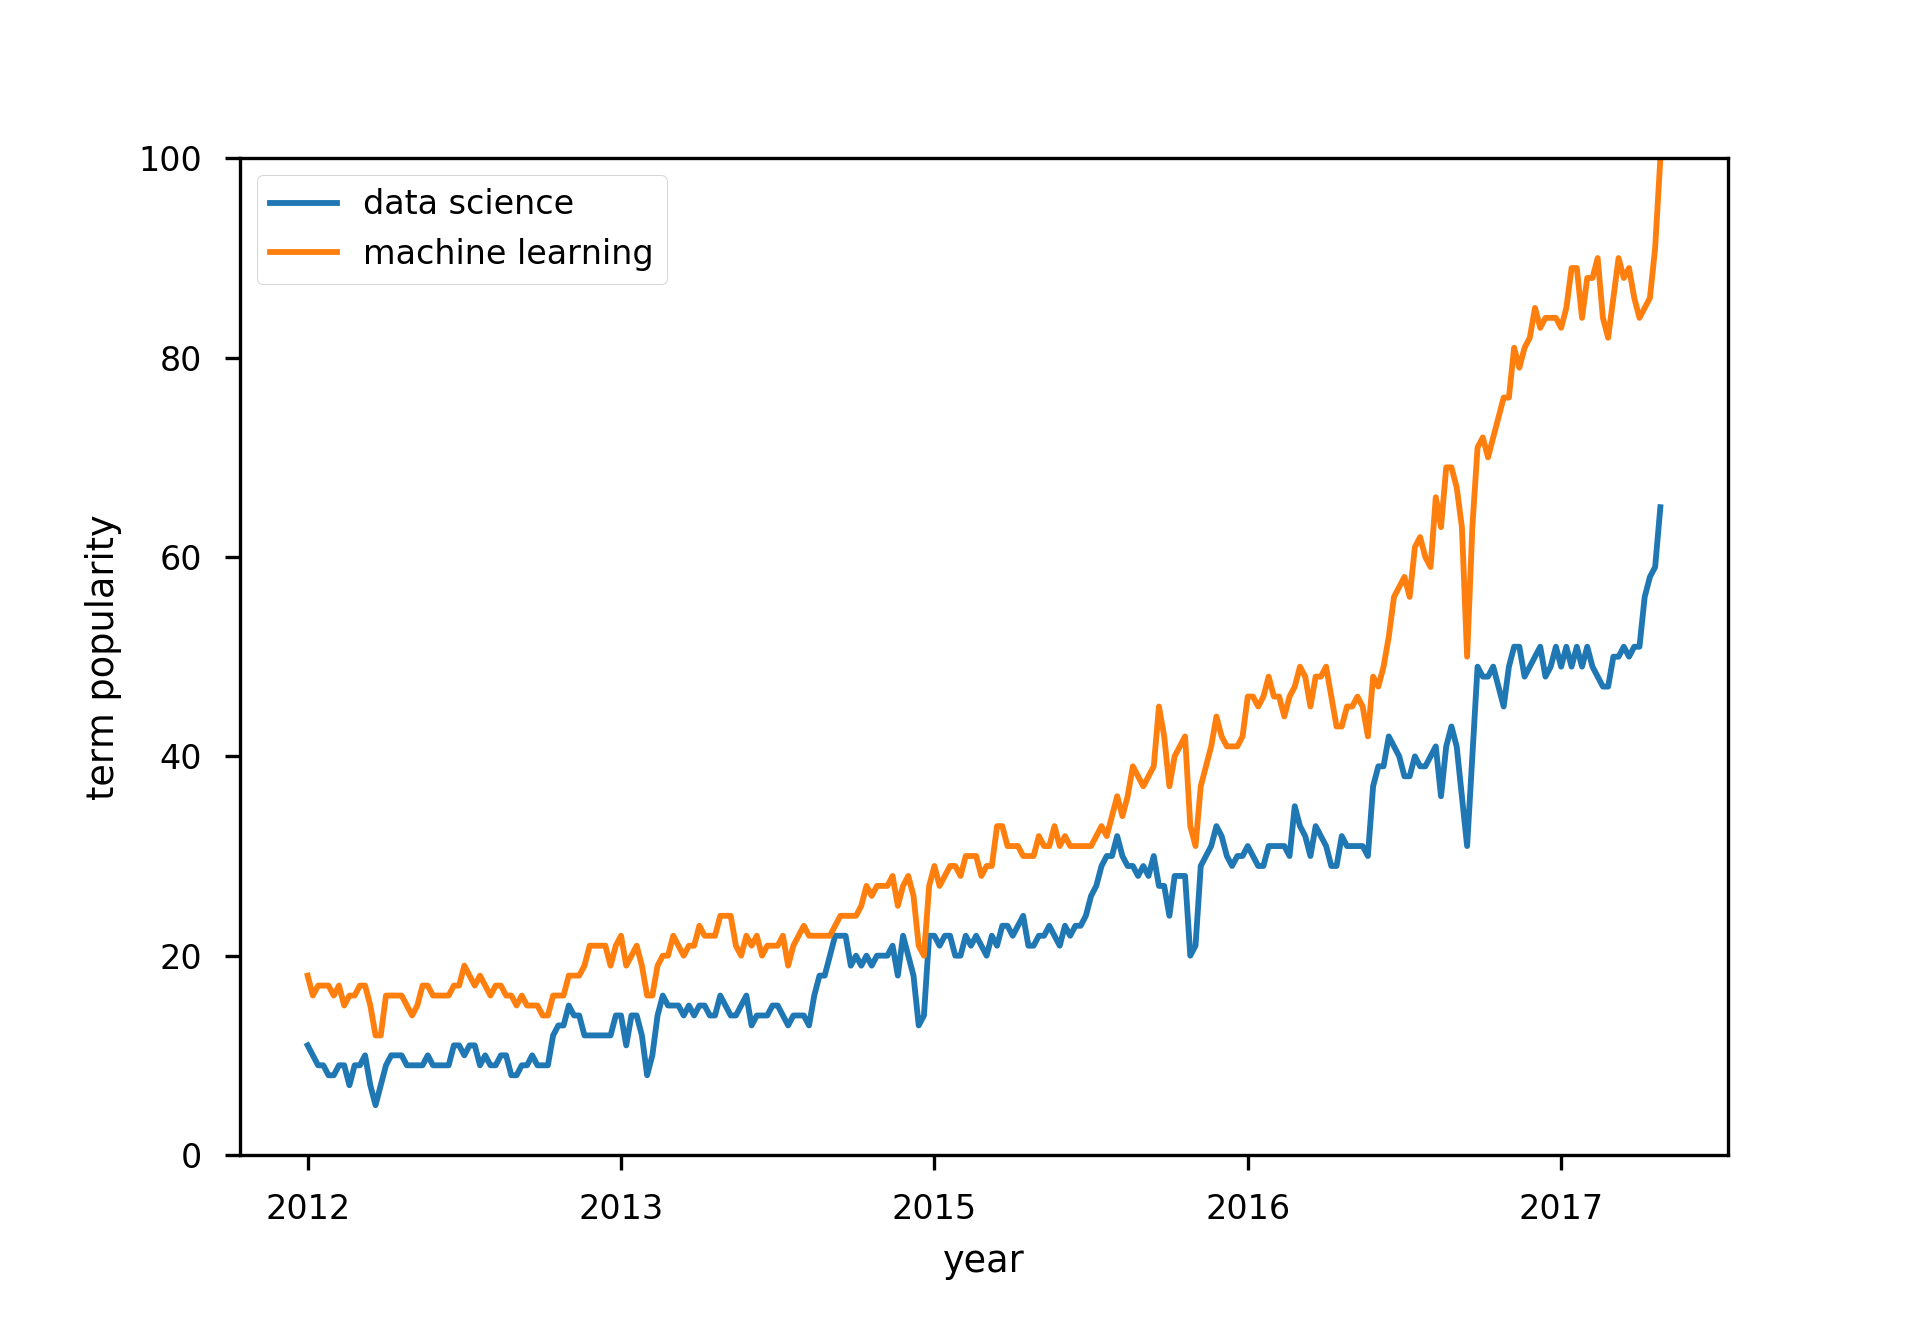
\includegraphics[width=0.8\textwidth]{part1/google_trends_MLDS.png}
  \caption{The Internet popularity over the past five years of two terms: \textit{data science} and \textit{machine learning}. The vertical axis represents the number of Google searches of an input term normalized with respect to its maximum (source: Google Trends).} \label{fig:google_trend_ML}
\end{figure}

A partial explanation to this phenomenon can be found in a recent article published on Science~\cite{appenzeller2017revolution}, where the authors observed how the explosion of modern data collection abilities is leading the human kind toward another \textit{scientific revolution}.
Biomedical applications are prototypical in this sense. For instance, the volume of the raw data acquired from a genome sequencer for a single \ac{DNA} has a volume of approximately 140 GB~\cite{marx2013biology}. Another example can be the 3D reconstruction of cardiac MRI acquisition which need around 20 GB for a single human heart, or the 3D \ac{CT} scan which has a volume in the order of GB for each patient. Several more examples can be given. It has been estimated that an average hospital currently stores more than 665 TB of data that need to be analyzed and understood.
%the typical resolution of MRI images is currently $512 \times 512$
Such massive amounts of data have long overwhelmed human analysis and insights potential. This makes ML a key element for clinicians and scientists that try to make sense of large-scale observations.

But, what is \textit{machine learning}? And how does it differ from statistics?

A unique answer to this question may not be easy to provide. In fact, ML can be defined in different ways and from several standpoints. Let's see three remarkable examples.

\begin{enumerate}
  \item Kevin P. Murphy in its \emph{Machine Learning - A Probabilistic Perspective}~\cite{murphy2012machine} defines machine learning as follows.

  \begin{displayquote}
  "[...] \emph{a set of methods that can automatically detect patterns in data, and then use the uncovered patterns to predict future data, or to perform other kinds of decision making under uncertainty} [...]"
  \end{displayquote}

  \item Trevor Hastie, a well-known applied statistician, in a famous seminar\footnote{part of Data Science @ Stanford Seminar series (source: \url{https://goo.gl/UFgqxU})}, held in October 2015 at the Stanford University, gave the following three definitions.

  \begin{displayquote}
    \begin{itemize}
      \item[] \emph{{\bf Machine Learning} constructs algorithms that can learn from data.}
      \item[] \emph{{\bf Statistical Learning}  is a branch of applied statistics that emerged in response to machine learning, emphasizing statistical models and assessment of uncertainty.}
      \item[] \emph{{\bf Data Science}  is the extraction of knowledge from data, using ideas from mathematics, statistics, machine learning, computer science, engineering...}
    \end{itemize}
  \end{displayquote}

  \item Carl E. Rasmussen in the preface of its renowned \emph{Gaussian Processes for Machine Learning}~\cite{rasmussen2006gaussian} introduces the difference between statistics and ML as follows.

  \begin{displayquote}
    "\emph{in statistics a prime focus is often in understanding the data and relationships in terms of models giving approximate summaries such as linear relations or independencies. In contrast, the goals in machine learning are primarily to make predictions as accurately as possible and to understand the behaviour of learning algorithms}"
  \end{displayquote}

\end{enumerate}

It looks like each author, according to his background, expertise and experience, provides a slightly different definition of ML. Trying to summarize these three standpoints, we can say that \emph{ML is an interdisciplinary field that borrows the concept of data-driven model from statistics in order to devise algorithms that can exploit hidden patterns in current data and make accurate predictions on future data}.

As of today ML is the workhorse of data science.


  \section{Supervised learning} \label{subsec:supervised_learning}

	  Humans are remarkably good at \emph{learning by examples}. When a kid is taught what a pencil looks like, he will be capable of understanding the concept of pencil from a limited number of guided observations. Similarly, when future radiologists are trained to distinguish between healthy tissues from tumors in MRI scans, they will be provided with several annotated biomedical images from which they will be able to generalize.
	  The applied learning paradigm is characterized by the presence of two key objects: \textit{data} and \textit{labels}. In the last example, the MRI scans are the data, and their annotations (\eg tumor \vs healthy tissue) are the labels.

	  Supervised learning is the branch of ML in which predictive models are trained on labeled data. In the ML jargon, and in this thesis, one usually refers to \textit{data} as collections of \textit{samples} described by an arbitrarily large number of \textit{predictors} (\textit{features}) that are used as \textit{input} in a training process having labels as \textit{output}.

	  Input samples throughout this thesis are represented as $d$-dimensional vectors $\bm{x}$ belonging to an input space $\mathcal{X}$, where typically $\mathcal{X}\subseteq\mathbb{R}^d$ and labels are represented with the variable $y$ belonging to an output space $\mathcal{Y}$.
	  The nature of $\mathcal{Y}$ defines the learning task as \textit{binary classification} if  $\mathcal{Y} = \{-1,+1\}$, \textit{multiclass classification} if $\mathcal{Y} = \{1,2,\dots,k\}$,
	  \textit{regression} if $\mathcal{Y}\subseteq\mathds{R}$ and
	  \textit{vector-valued regression} if $\mathcal{Y}\subseteq\mathds{R}^k$.
	%  In the second part of this thesis each of these learning problems will be faced.
	  The remainder of this section summarizes the methods that are most relevant with the data-driven strategies adopted to tackle the biomedical data science challenges described in the second part of in this thesis.

	  Given a set of input-output pairs $\mathcal{D} = \{\bm{x}_i, y_i\}_{i=1}^n = (X, \bm{y})$, supervised learning methods aim at finding a function of the inputs $f(\bm{x})$ that approximates the output $y$. This translates into the minimization problem defined in Equation~\eqref{eq:loss}.

	  \begin{equation}\label{eq:loss}
	    \argmin_f \frac{1}{n}\sum_{i=1}^n L(f(\bm{x}_i),y_i) %+ \lambda R(f)
	  \end{equation}

	  The loss function $L(f(\bm{x}),y)$ can be seen as a measure of \textit{adherence} to the available training data. Several loss functions for regression and classification problems were proposed; Table~\ref{tab:losses} defines the most commonly adopted in biomedical studies while their visual representation is presented in Figure~\ref{fig:loss}.
	  Choosing the appropriate loss function for the problem at hand is crucial and there is no trivial solution for this problem.
	  Different choices for $L(f(\bm{x}),y)$ identifies different learning machines, that are known under different names. The most popular methods will be presented in the next few sections.
	  % \todo{Different choices for the loss function imply different ML model, see the remainder of this section + this is possibly ill-posed}

	  \begin{figure}[!h]
	  	\centering
	  	\subfloat[]{%
	  		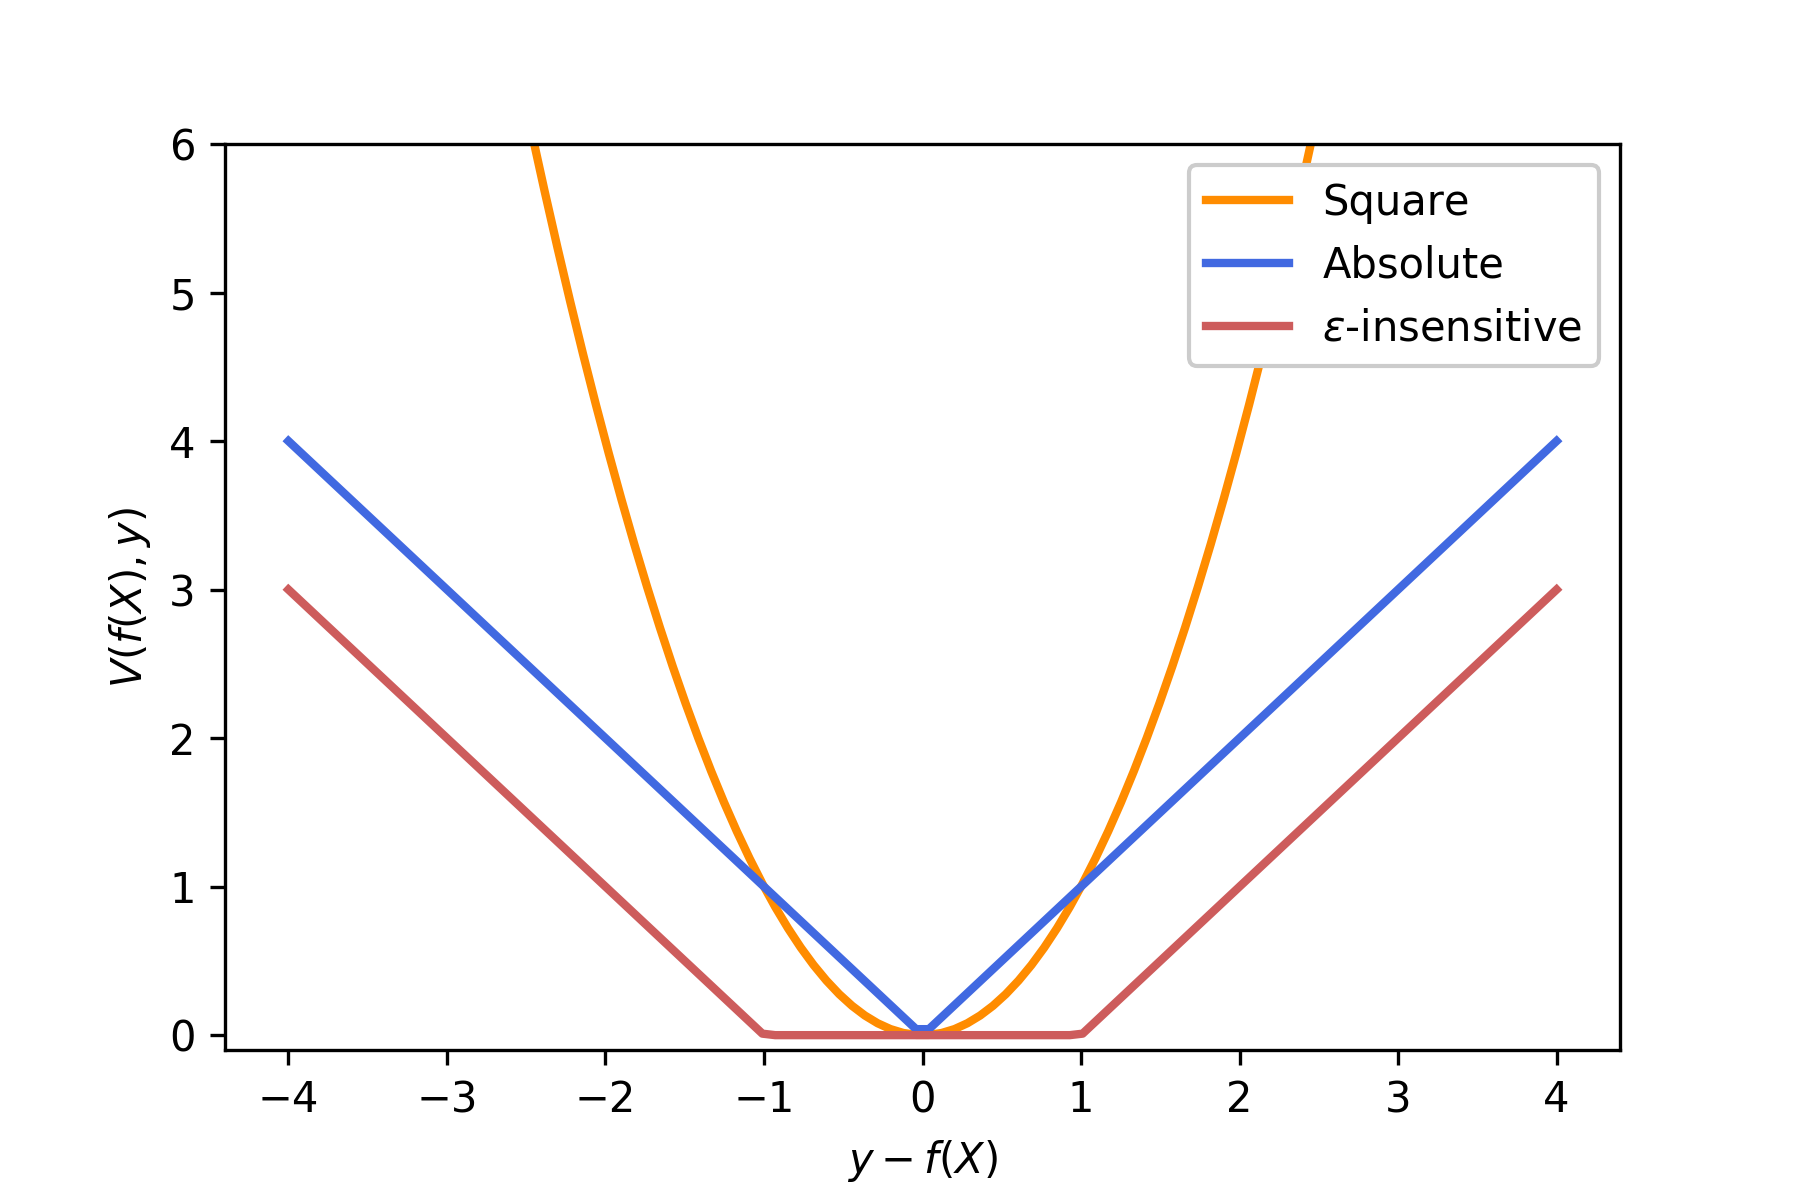
\includegraphics[width=0.5\textwidth]{part1/regression_losses.png}
	  		\label{fig:regression}%
	  	}%
	  	% \hfill%
	  	\subfloat[]{%
	  		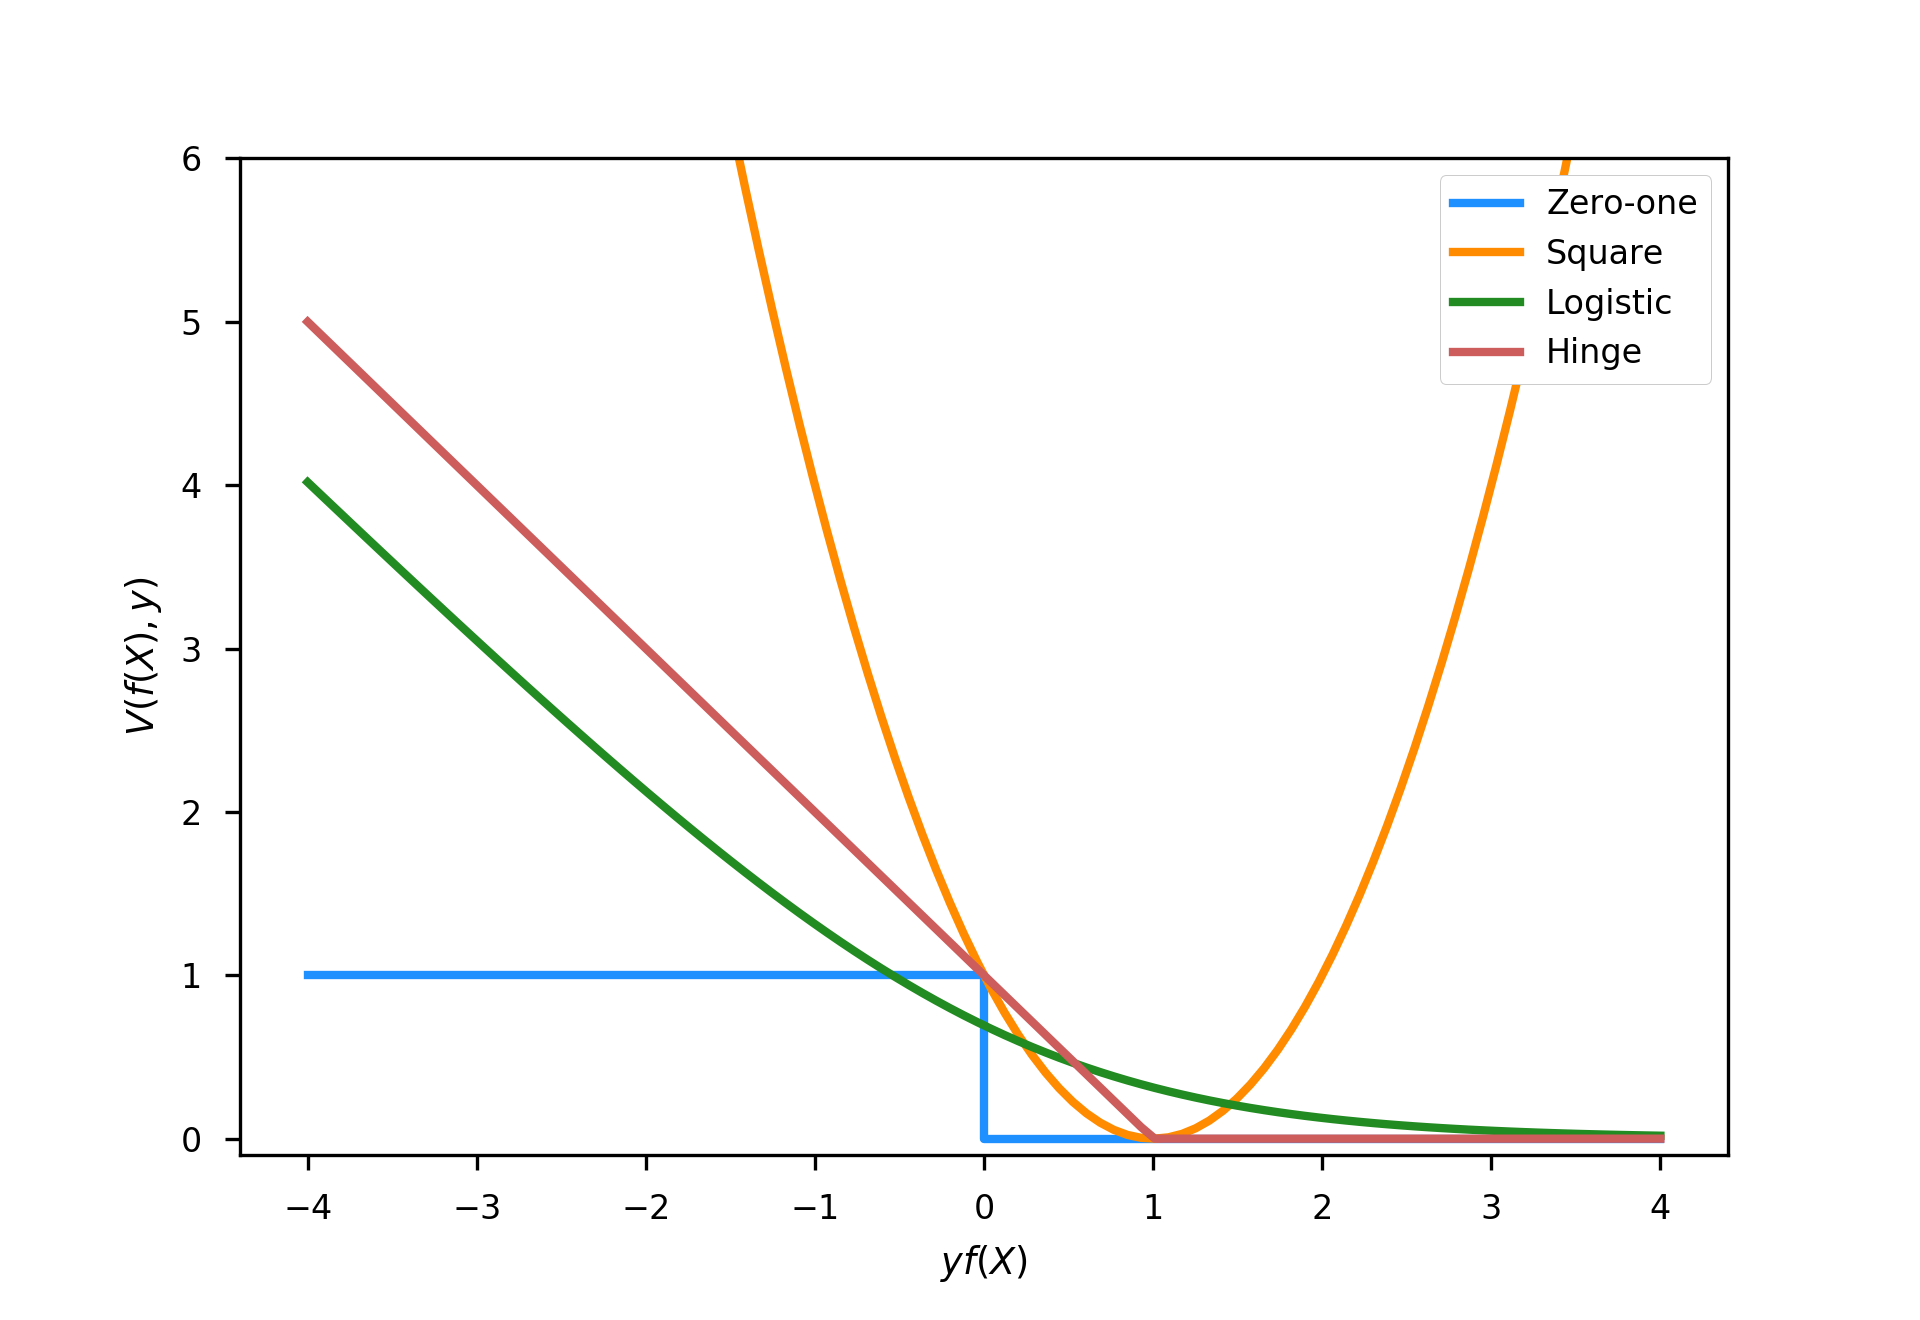
\includegraphics[width=0.5\textwidth]{part1/classification_losses.png} \label{fig:classification}
	  	}%
	  	\caption{An overview on the most common loss functions for regression (a) and classification (b) problems plotted against the corresponding prediction error.}\label{fig:loss}
	  \end{figure}


	  \begin{table}[!h]
	  	\centering
	  	\caption{Definition of the loss functions for regression (top) and classification (bottom) problems represented in Figure~\ref{fig:loss}.}\label{tab:losses}
	  	\begin{tabular}{@{}ll@{}ll@{}}
	  		\toprule
	  		Loss function & $L(f(\bm{x}),y)$  & Learning problem           \\ \midrule
	  		Square                   & $(y - f(\bm{x}))^2$ & regression \\
	  		Absolute                 & $|y - f(\bm{x})|$ & regression   \\
	  		$\epsilon$-insensitive   & $\begin{cases}
	  		0 & \text{if } |y-f(\bm{x})| < \epsilon\\
	  		|y-f(\bm{x})| - \epsilon & \text{otherwise}
	  		\end{cases} $        & regression                 \\
	  		\midrule
	  		Zero-one               & $\begin{cases}
	  		0 & \text{if } y = f(\bm{x})\\
	  		1 & \text{otherwise}
	  		\end{cases}$ & classification \\
	  		Square                 & $(1 - yf(\bm{x}))^2$ & classification  \\
	  		Logistic                 & $\log(1 + e^{-yf(\bm{x})})$ & classification  \\
	  		Hinge                 & $|1 - yf(\bm{x})|_+$ & classification  \\
	  		Exponential & $e^{- yf(\bm{x})}$ & classification \\
	  		\bottomrule
	  	\end{tabular}
	  \end{table}

	   % rubare da BIB
	  % In its most classical definition, the aim of modeling is to infer some unknown structure underlying the data.
	  Identifying a reliable data-driven model can be a very tricky task. Many unwanted and concurrent factors may be misleading and the solution may have poor predictive power for several reasons.
		Including:
		\begin{enumerate}
			\item the acquisition devices may introduce random fluctuations in the measures;
			\item the amount of collected samples $n$ may be small with respect to the number of observed variables $d$;
			\item the measured variables may not be representative of the target phenomenon.
	  \end{enumerate}
		From a modeling standpoint, every combination of the factors above can be seen as \textit{noise} affecting the data.
		Precautions in the model formulation process must be taken in order to achieve solutions that are insensitive to small changes in the input data and that are, in general, \textit{robust} to the noise effect.

		Considering a ML model ($\hat f$) fitted on a collection of data ($\mathcal{D}$), the most desirable property of $\hat f$ is that it should be able to achieve good prediction performance not only on $\mathcal{D}$, but also on all the future, therefore unseen, data points $\mathcal{D}'$.
		In other words, assuming that the samples in $\mathcal{D}$ are affected by some kind of random\footnote{here with \textit{random} we mean "\textit{uncorrelated with the input-output relationship}"} component, $\hat f$ should be able to learn a predictive function that does not \textit{follow the noise}, but rather models the true input-output relationship.
		In ML, a model that fits well $\mathcal{D}$ but performs poorly on $\mathcal{D}'$ is said to be \textit{overfitting}.

	  \begin{figure}[!h]
	  	\centering
	  	\subfloat[]{%
	  		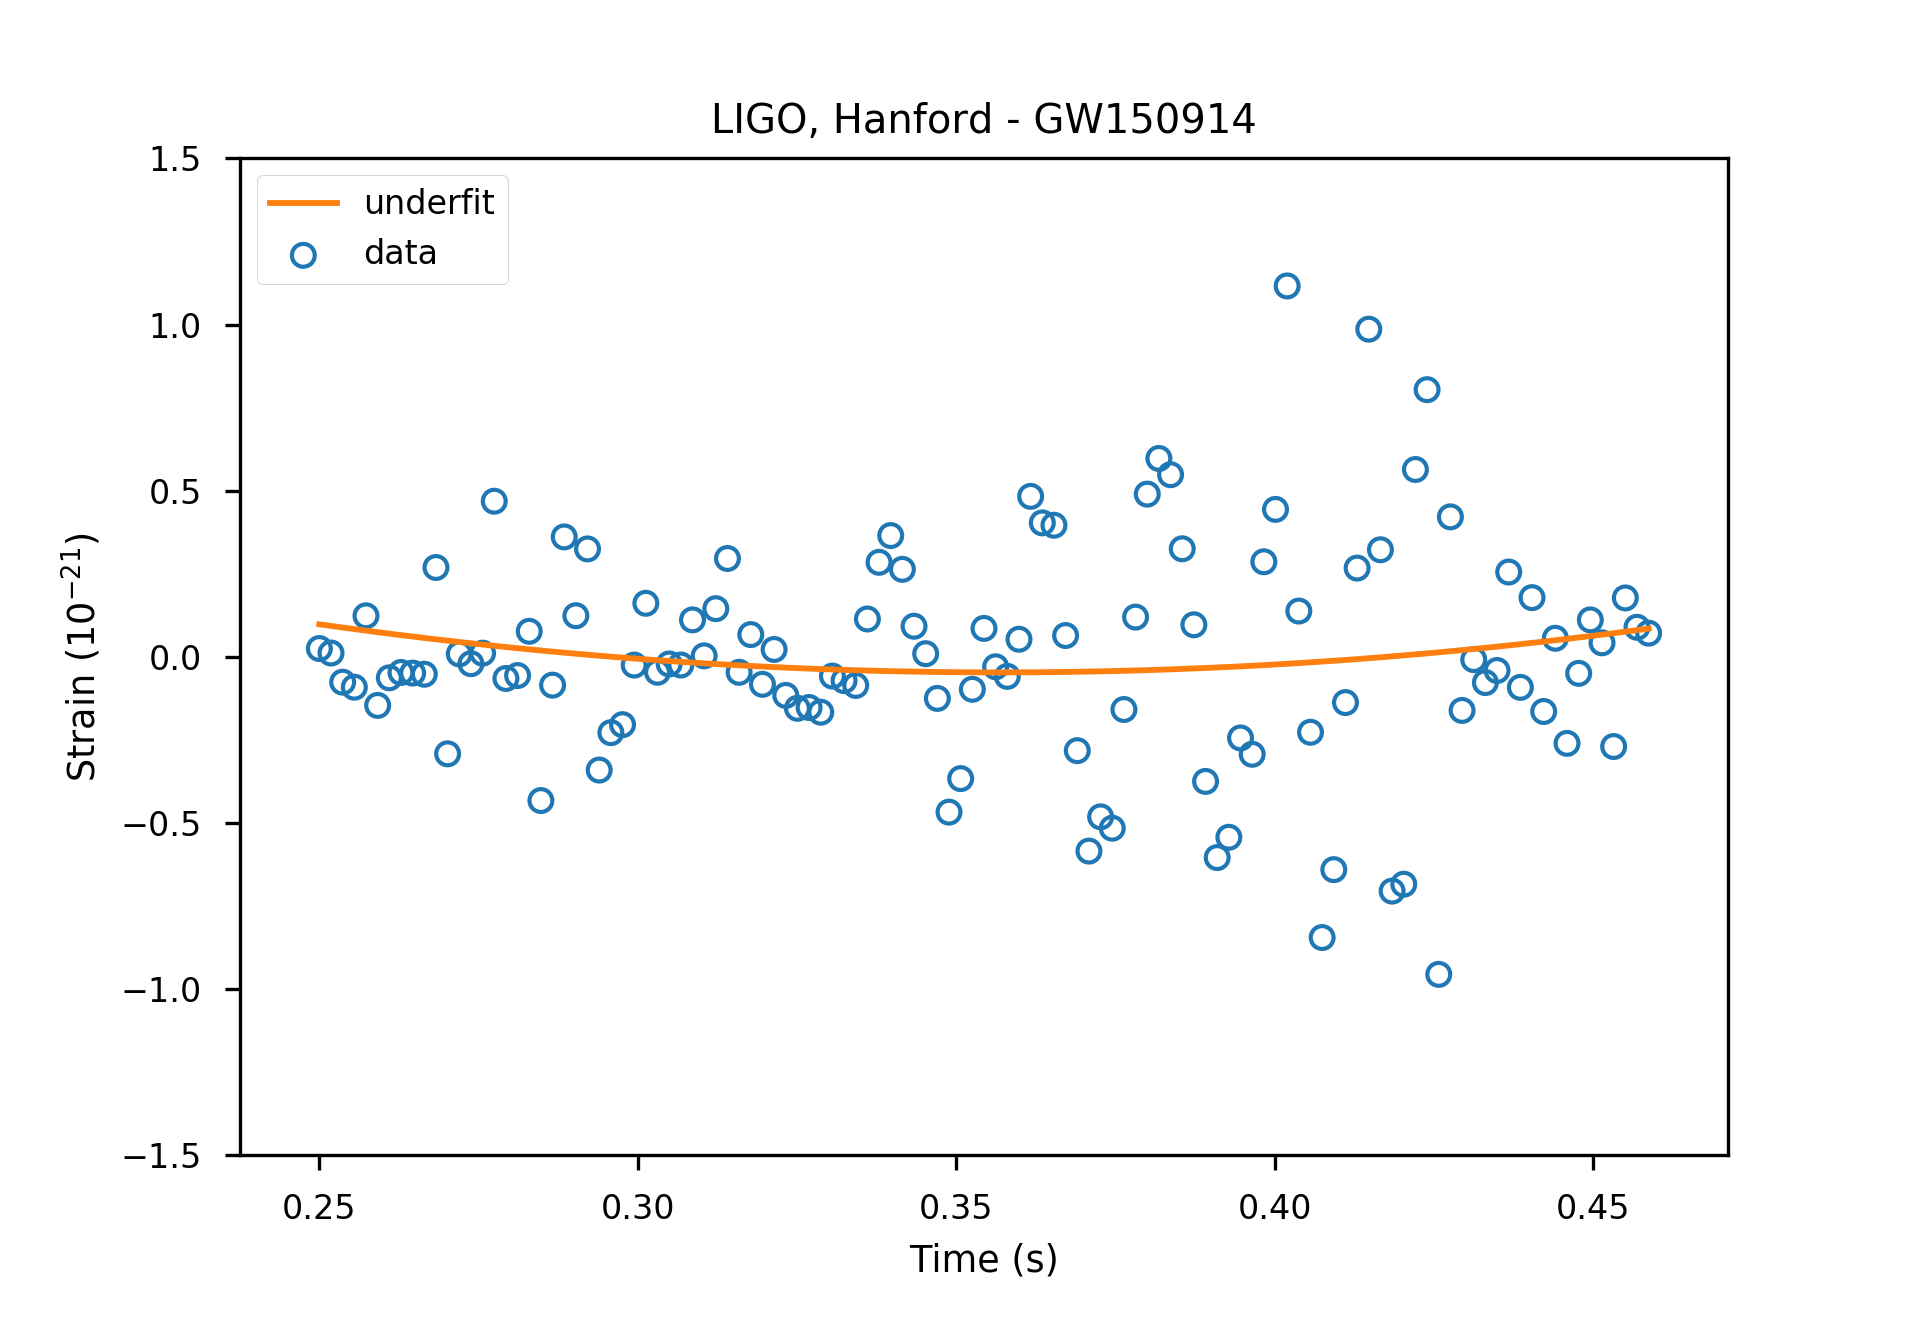
\includegraphics[width=0.5\textwidth]{part1/0_regression_underfit.png}
	  		\label{fig:regression}%
	  	}%
	  	%\hfill%
	  	\subfloat[]{%
	  		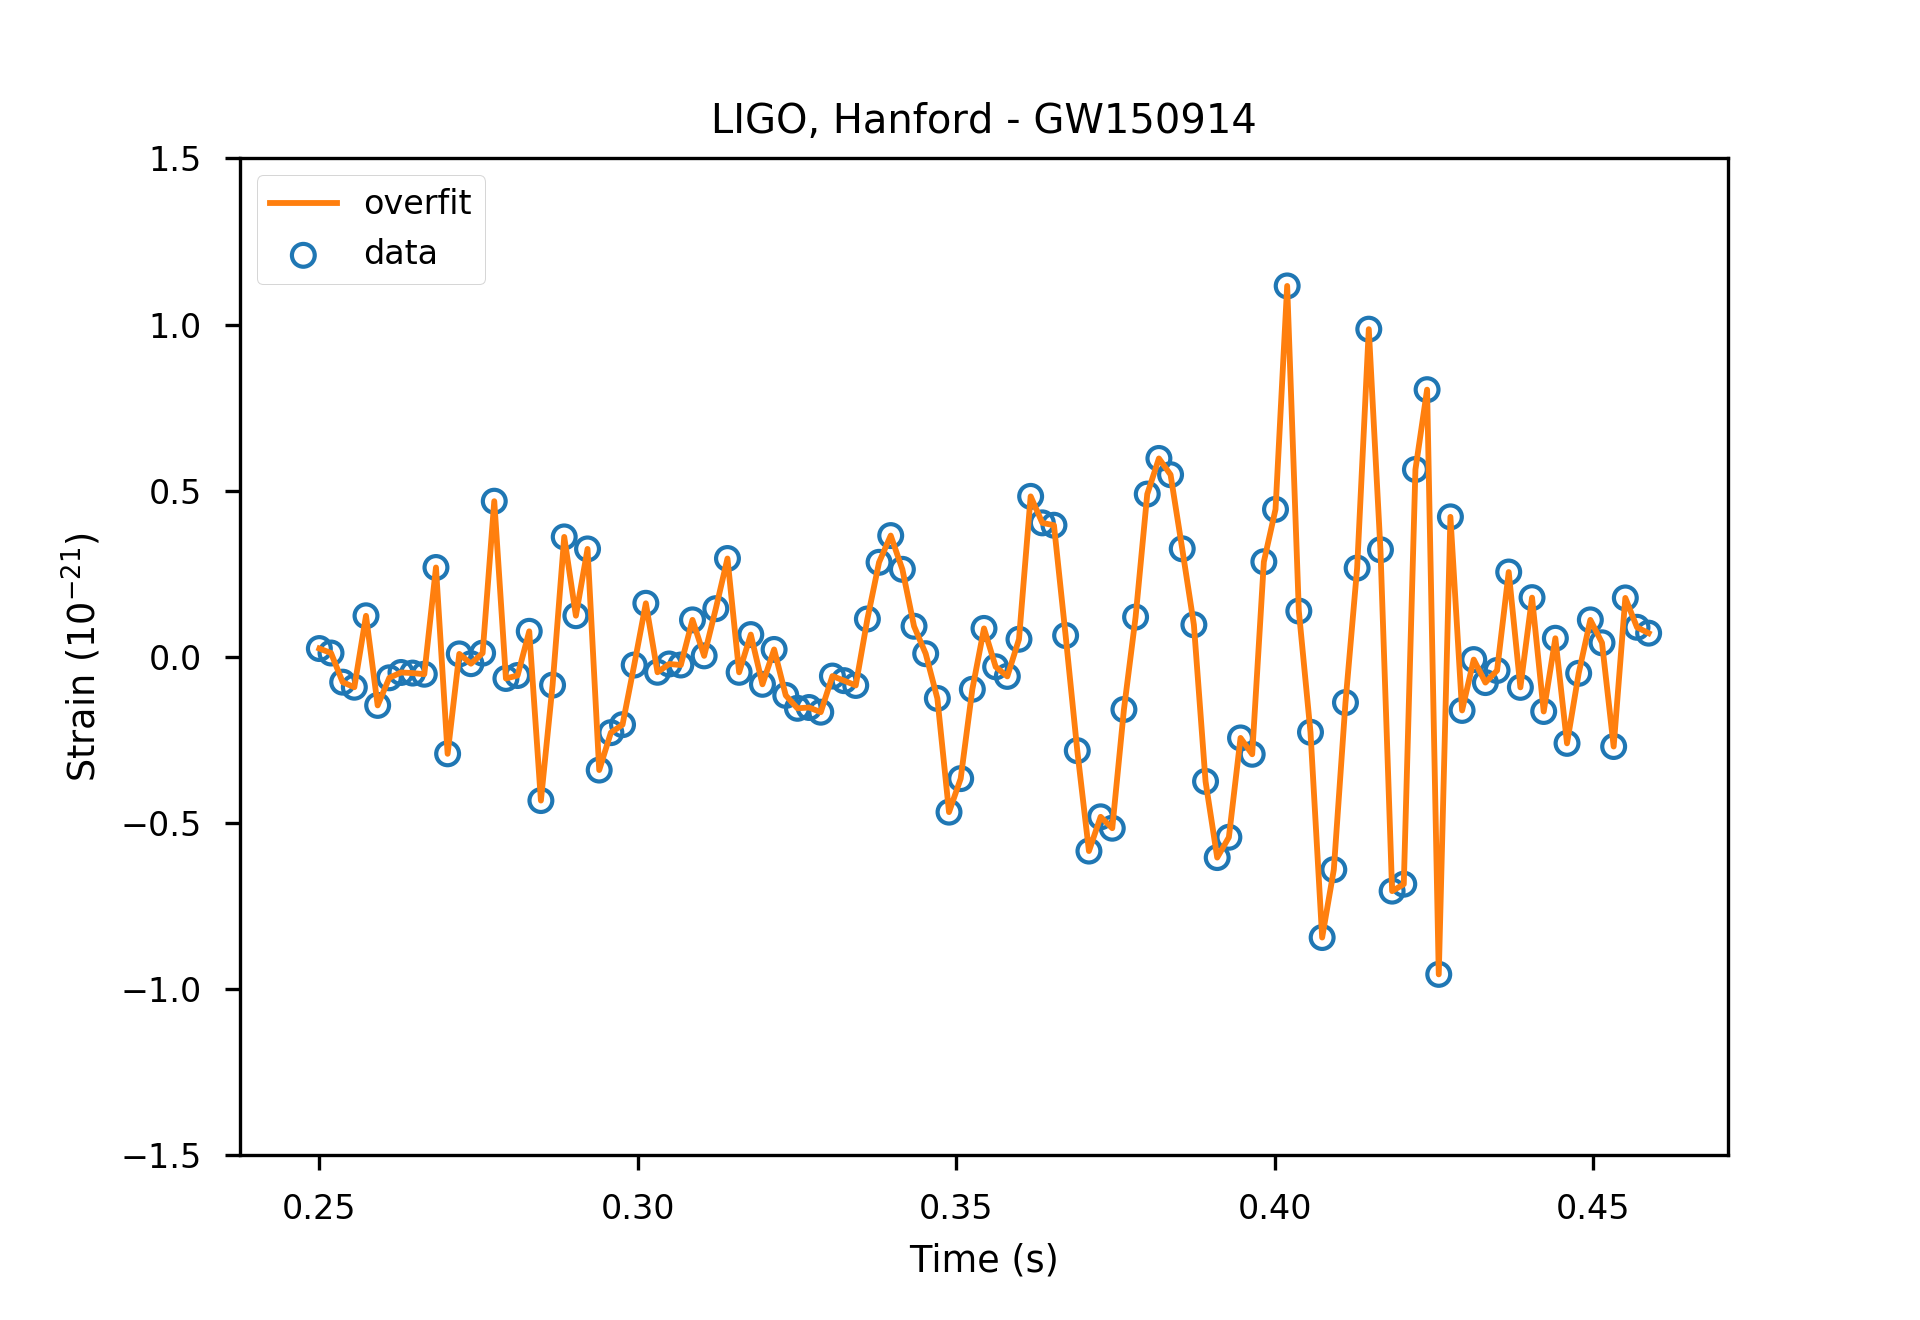
\includegraphics[width=0.5\textwidth]{part1/1_regression_overfit.png}
	  		\label{fig:regression}%
	  	}%
	      \hfill%
	  	\subfloat[]{%
	  		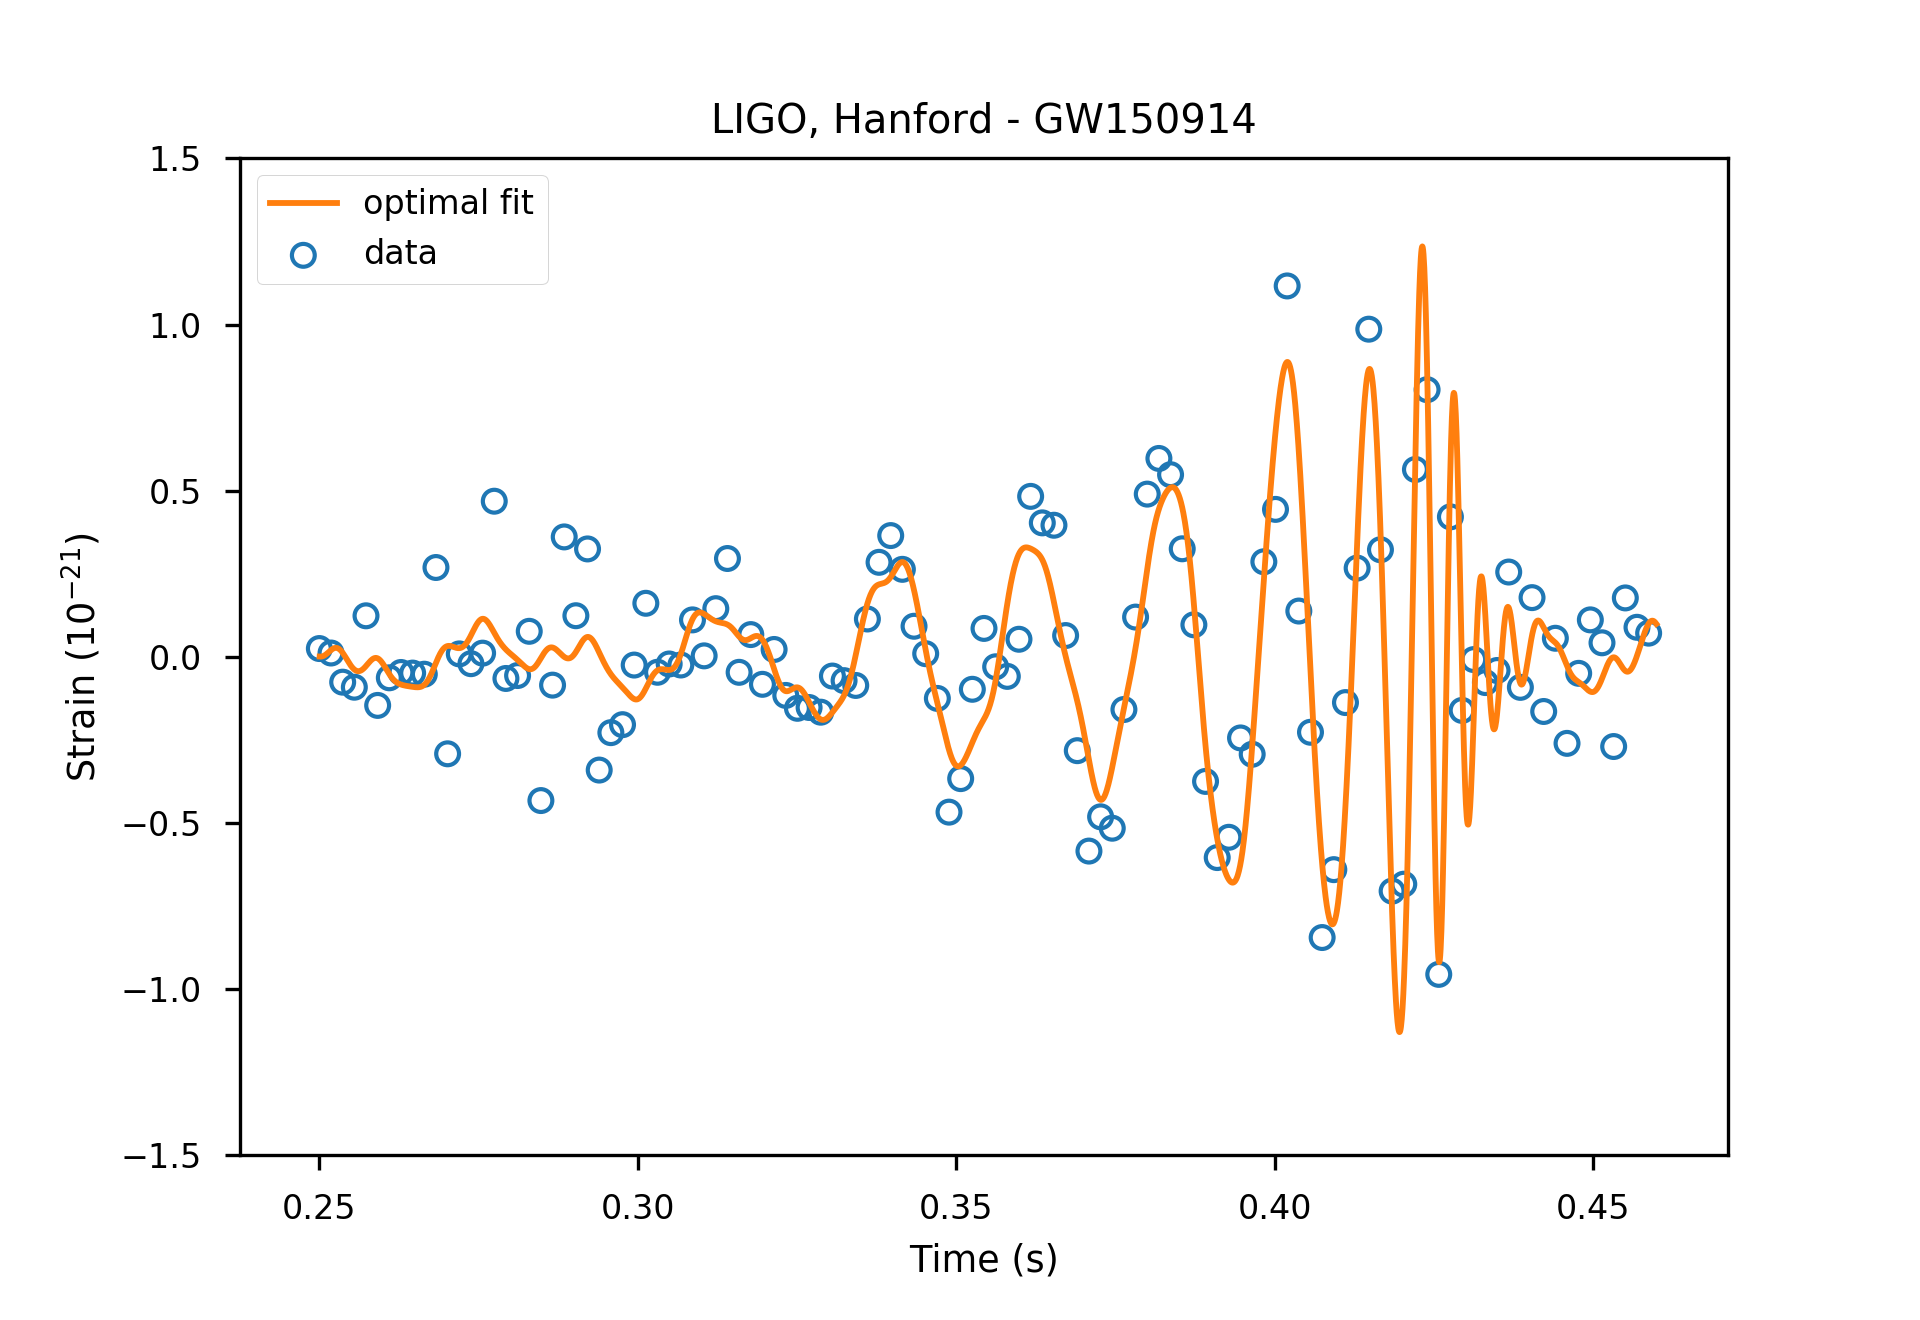
\includegraphics[width=0.5\textwidth]{part1/2_regression_fit.png}
	  		\label{fig:regression}%
	  	}%
	  	\caption{An example of underfit (a), overfit (b) and optimal fit (c) for a regression problem. The data are a downsampled version ($f_s = 546~Hz$) of the first observation of gravitational waves from a binary black hole merger detected on September 14\textsuperscript{th}, 2015, 09:50:45 {\sc utc} at LIGO Hanford (WA).}\label{fig:regression_fit}
	  \end{figure}

	  \begin{figure}[!h]
			\centering
			\subfloat[]{%
				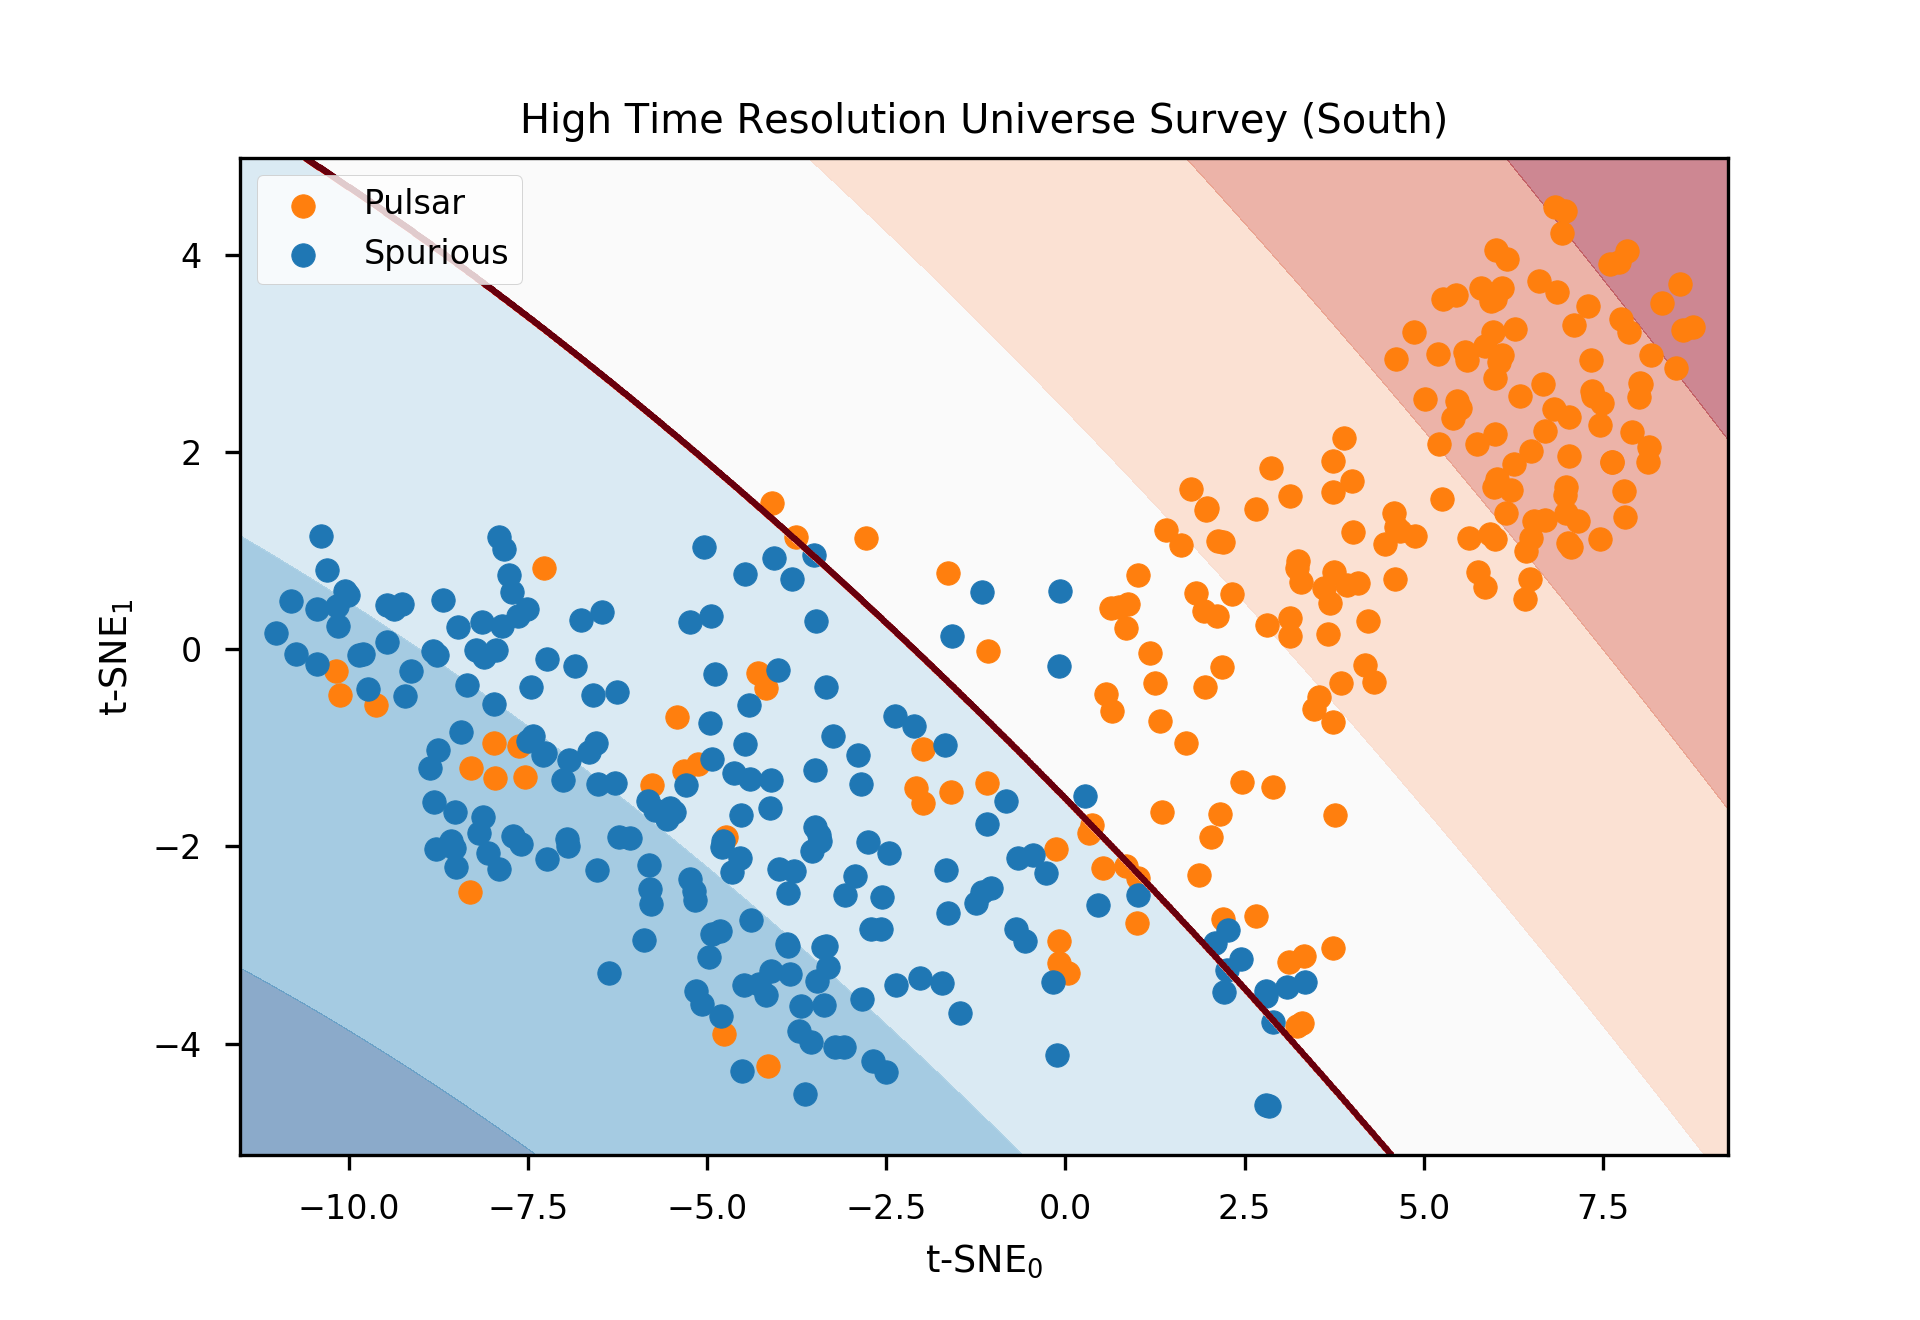
\includegraphics[width=0.5\textwidth]{part1/0_classification_underfit.png}
				\label{fig:regression}%
			}%
			%\hfill%
			\subfloat[]{%
				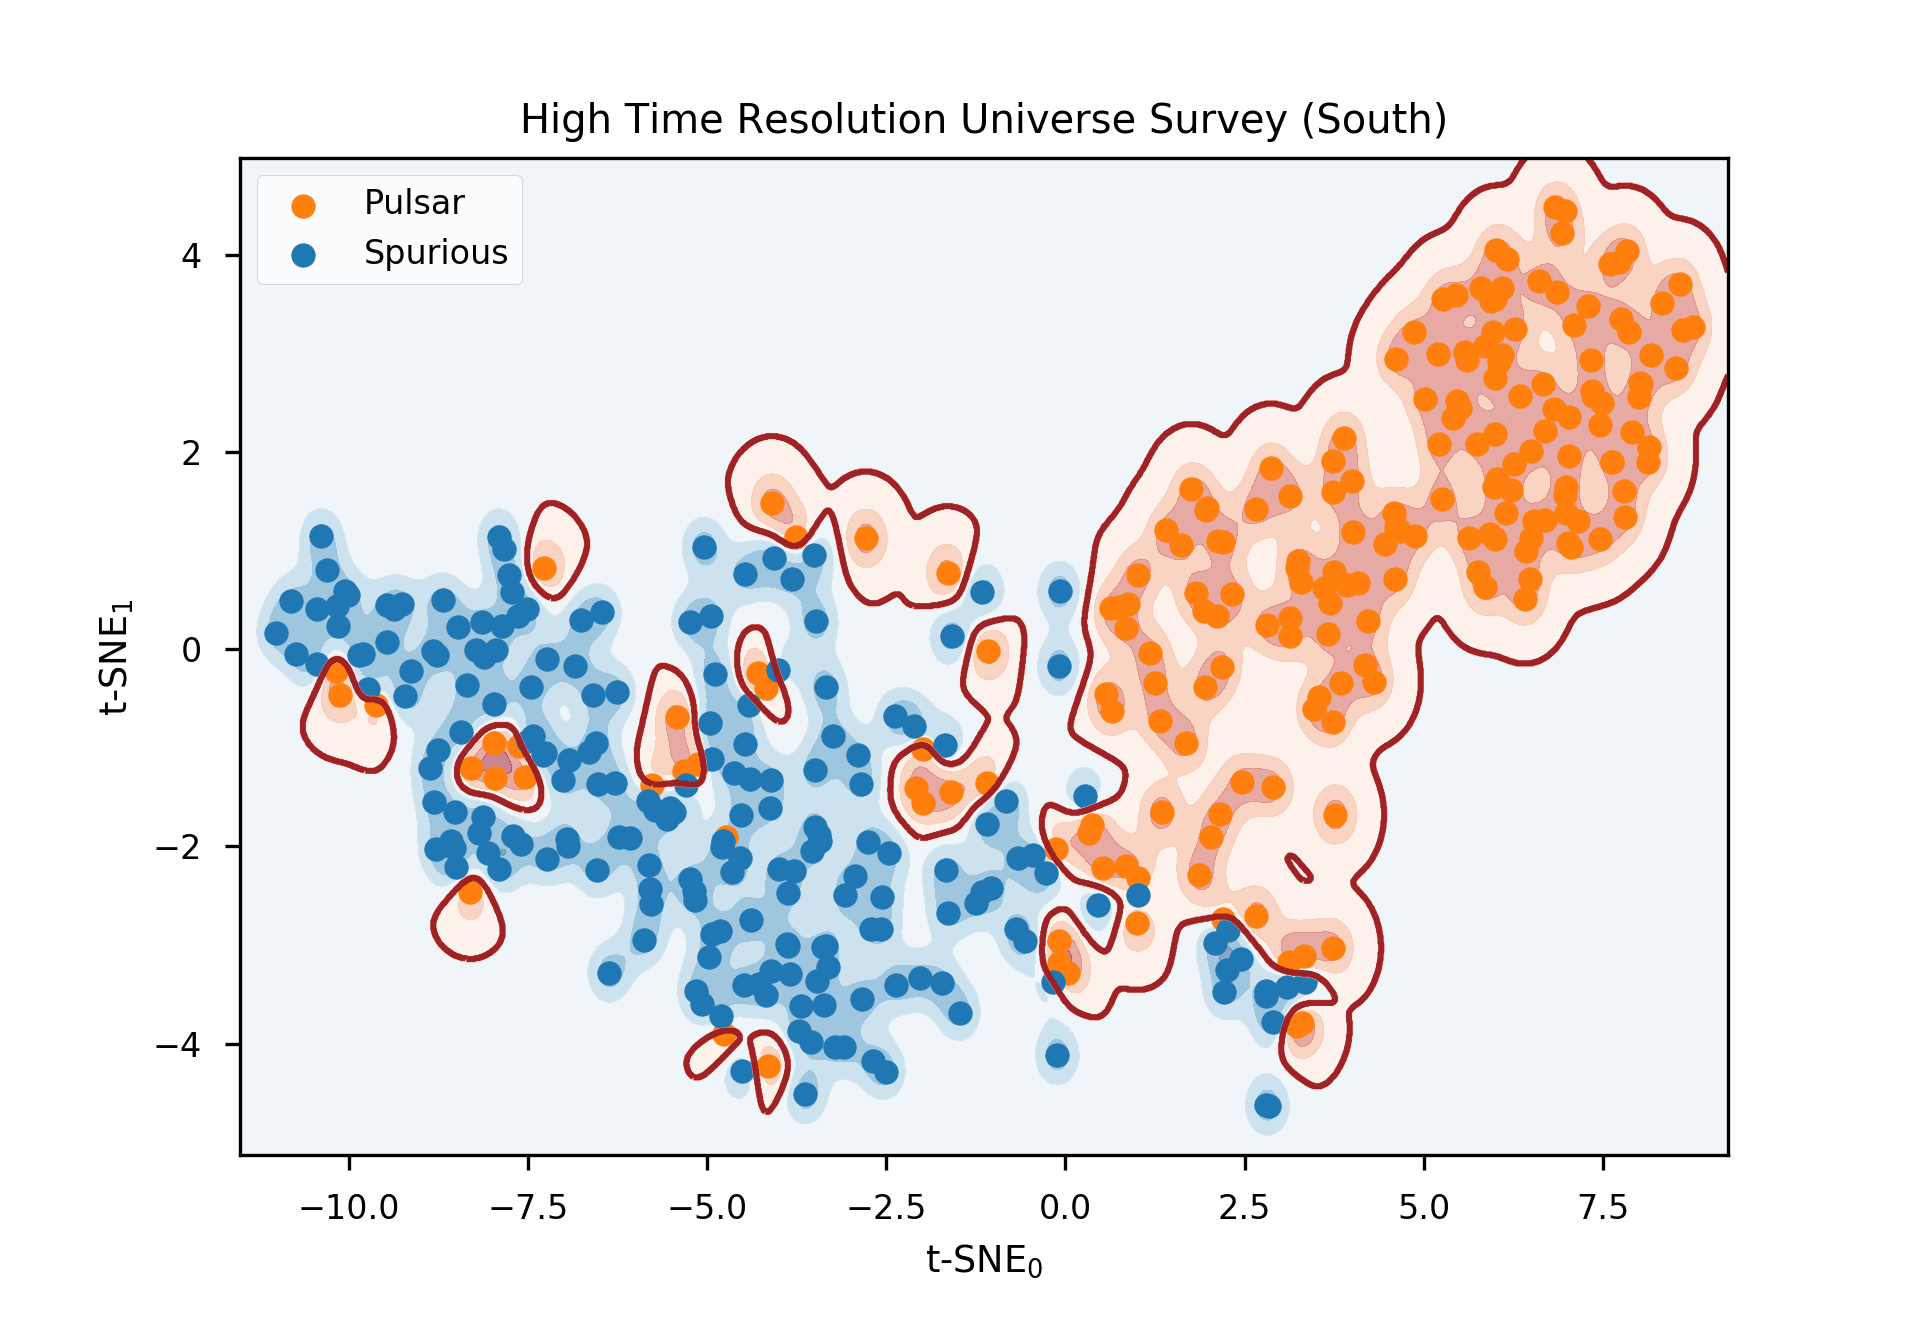
\includegraphics[width=0.5\textwidth]{part1/1_classification_overfit.png}
				\label{fig:regression}%
			}%
			\hfill%
			\subfloat[]{%
				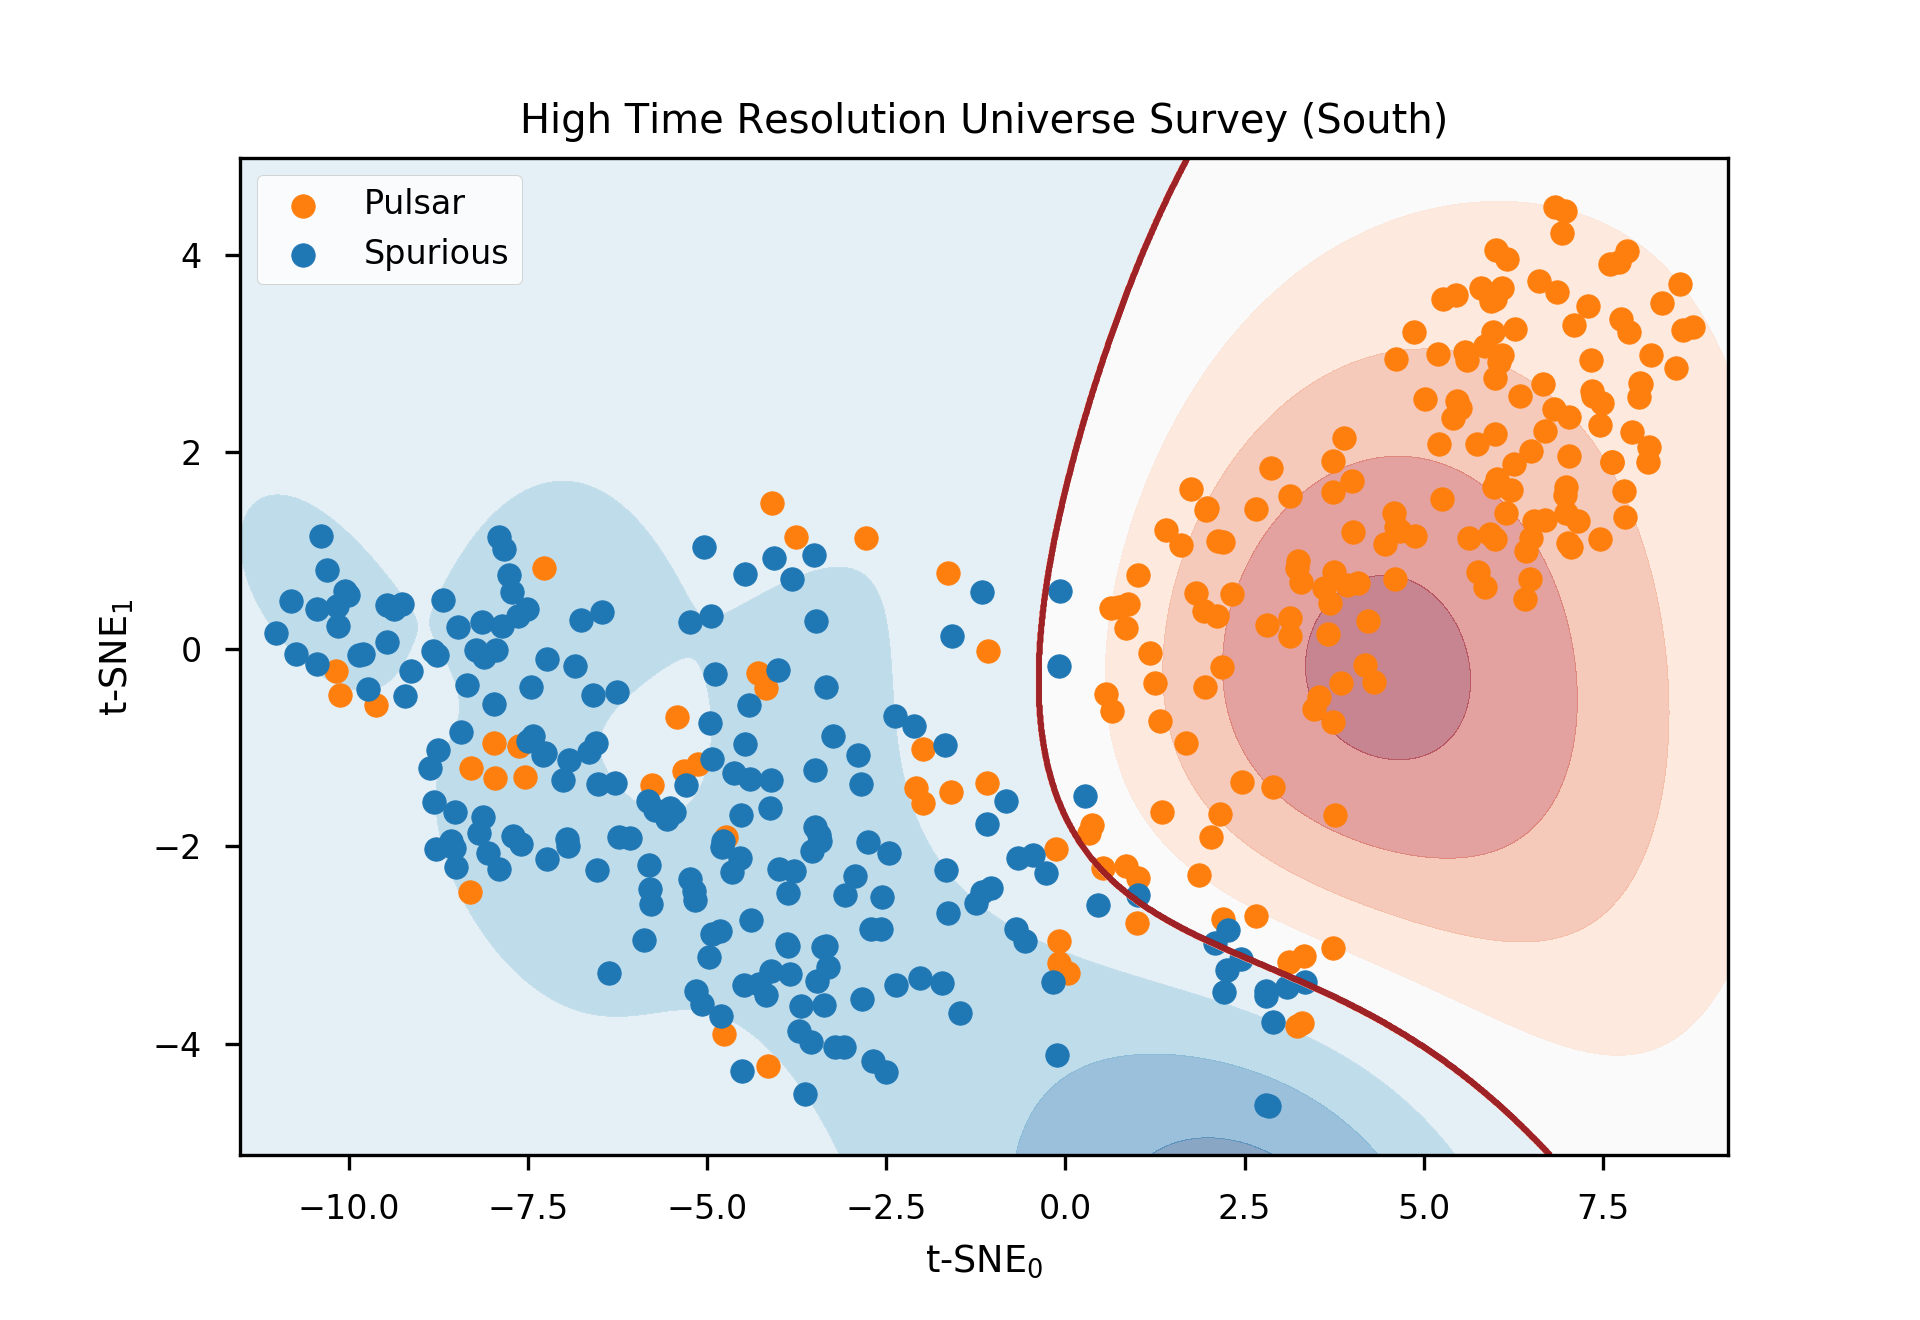
\includegraphics[width=0.5\textwidth]{part1/2_classification_fit.png}
				\label{fig:regression}%
			}%
			\caption{An example of underfit (a), overfit (b) and optimal fit (c) for a binary classification problem. Each data point is a pulsar candidate randomly sampled from the High Time Resolution Universe Survey (South) dataset. The data are standardized and their dimensionality is reduced by the t-SNE algorithm~\cite{van2008visualizing}. }\label{fig:classification_fit}
	  \end{figure}


%	    Real-world data collections can be heavily affected by random noise,
%	    As the biomedical world is the the main area of interest of this thesis (see Section~\ref{sec:challenges_biomedical}),
%	    The most widely adopted common strategy to build predictive models out of noisy data is called \textit{regularization}.
        In ML literature, \textit{regularization} is the most important countermeasure to overfitting and it is widely adopted, under several forms, to build predictive models out of noisy data.

	    The original contribution of this phd thesis mainly relies on the application of data science and ML concepts to noisy domains. Therefore, regularization strategies are of primary interest in this discussion.
	    For each learning algorithm described, particular emphasis will be put on the relevant regularization strategies.
	    In its broader definition \textit{regularization} can be seen as the process of introducing additional information in order to solve a possibly ill-posed problem.
			As shown in Equation~\eqref{eq:losspen}, this is typically translated in the use of a regularization penalty $\mathcal{R}(f)$, controlled by a regularization parameter $\lambda$ \cite{tikhonov1963solution, evgeniou2000regularization}.

	     \begin{equation}\label{eq:losspen}
	    	\argmin_{f \in \mathcal{F}} \frac{1}{n}\sum_{i=1}^n L(f(\bm{x}_i),y_i) + \lambda \mathcal{R}(f)
	    \end{equation}

			% The expected result is a function that fits the training data while having good generalization properties, \ie accurate predictions on previously  \textit{unseen} test data \cite{hastie2009elements}.
			Choosing different $\mathcal{R}(f)$ implies inducing different effects on the solution and it also leads to the definition of different learning machines (see Section~\ref{subsec:regularization_methods}).
			With the regularization parameter $\lambda$ it is possible to control the trade-off between adherence to the training data and strength of the effect induced by the $\mathcal{R}(f)$.
			As an example, we can think of using a penalty that induces smoothness, such as the $\ell_2$-norm, or sparsity, such as the $\ell_1$-norm, in the solution.
			A pictorial representation of a learning machine working in overfitting, underfitting and optimal fitting regime in a regression and a classification case can be seen in
			Figure~\ref{fig:regression_fit}~\footnote{source \url{https://losc.ligo.org/events/GW150914/}}
			and
		  Figure~\ref{fig:classification_fit}~\footnote{source \url{https://archive.ics.uci.edu/ml/datasets/HTRU2}}, respectively.


	%    The regularization penalty $R(f)$ imposes stability on the expected function exploiting the available prior knowledge on the problem~\cite{tikhonov1963solution}. More details on $R(f)$ will be given in the next section.

	    Supervised learning machines may rely on very different mathematical backgrounds such as generalized linear models, nonlinear deep neural networks, kernels, trees, ensemble of trees, \etc. Nevertheless, disregarding their nature, they all share the common structure defined in Equation~\eqref{eq:losspen}.
	    The solution of this problem can be achieved either by Empirical (or Structured) Risk Minimization (\ac{ERM}) either by Maximum Likelihood/A Posteriori (\ac{MLE}/\ac{MAP}) Estimation. See Appendix~\ref{appendix:A} for more details on this two strategies, and their connection.

	    \subsection{Regularization methods} \label{subsec:regularization_methods}
	    Regularization methods is a broad class of models that include linear and nonlinear techniques for both regression and classification. The main characteristic of the methods falling in this class, is that they are particularly straightforward to express as in Equation~\eqref{eq:losspen}. In fact, as described in~\cite{evgeniou2000regularization}, most of them are simply identified by the use of one loss function $L(f(\bm{x}), y)$ and one, or more, regularization penalty $\mathcal{R}(f)$.

	    In the following sections an overview of the most popular regularization methods is presented.

			%%%%%%%%%%%%%%%%%%%%%%%%%%%%%%%%%%%%%%%
			\subsubsection{Ordinary least squares} \label{sec:ols}
			We start this discussion focusing on linear models $\hat y = f(\bm{x})=\bm{x}^T\bm{w}$ and taking into account the most popular loss function for regression problems: the square loss $L(\hat y, y) = (\bm{x}^T\bm{w}-y)^2$. The data fitting problem expressed in Equation~\eqref{eq:ols} is known as \textit{Ordinary Least Squares} (\ac{OLS}), or simply as \textit{linear regression}, and it does not include any regularization term.

			\begin{equation} \label{eq:ols}
				\bm{\hat w}_{\text{OLS}} = \argmin_{\bm{w} \in \mathbb{R}^d} \frac{1}{n} \sum_{i=1}^n (\bm{x}_i^T\bm{w} - y_i)^2 = \argmin_{\bm{w} \in \mathbb{R}^d} \frac{1}{n} \norm{X\bm{w} - \bm{y}}_2^2
			\end{equation}

			The minimization problem in Equation~\eqref{eq:ols} is convex and differentiable, hence its solution can be achieved in closed-form as
			$$
				\bm{\hat w}_{\text{OLS}} = (X^TX)^{-1}X^T\bm{y}
			$$
			or by iterative minimization routines such as (stochastic) gradient descent-like algorithms~\cite{boyd2004convex, sra2012optimization}. A pictorial representation of the solution of OLS can be seen in Figure~\ref{fig:w_ols}.

			Even though mainly used for regression, the square loss can be used to solve binary classification problems too (see Table~\ref{tab:losses}). In this case, the square loss can be rewritten as

			\begin{equation} \label{eq:margin_square_loss}
				(\bm{x}^T\bm{w}-y)^2 = (1-y \cdot \bm{x}^T\bm{w})^2
			\end{equation}

			exploiting the fact that the two classes are encoded with binary labels: $\bm{y} \in \{+1,-1\}^n$. For multiclass classification problems, strategies such as \textit{One-vs-One} (\ac{OVO}) or \textit{One-vs-All} (\ac{OVA}) can be adopted to reduce the problem to the binary classification setup~\cite{hastie2009elements}.

			In case of multiple tasks, the OLS approach can be extended to vector-valued regression tasks as well. In this case the least squares problem can be written as
			\begin{equation} \label{eq:vvr_ols}
				\begin{aligned}
				\hat W_{\text{OLS}}={} & \argmin_{W \in \mathbb{R}^{d \times k}} \frac{1}{n} \sum_{i=1}^n \sum_{t=1}^k (\bm{x}_i^T\bm{w}^t - y_i^t)^2  \\
				& =	\argmin_{W \in \mathbb{R}^{d \times k}} \frac{1}{n} \norm{XW - Y}_F^2
				\end{aligned}
			\end{equation}
			where $\norm{A}_F= \sqrt{\sum_{i=1}^n\sum_{t=1}^k |a_i^t|^2}$ is the \textit{Frobenius} norm (also known as  \textit{Hilbert-Schmidt} norm) and it can be considered as an extension of the $\ell_2$-norm to the matrix case.
			Lacking of appropriate regularization penalties, solving the problem in Equation~\eqref{eq:vvr_ols} corresponds to solving $k$ isolated regression problems, one for each task.
			This approach, even if theoretically legit, is rather uncommon in practical applications and a regularized version of Equation~\eqref{eq:vvr_ols} is typically preferred (see following sections).

			OLS is probably the most na\"ive prediction strategy, nevertheless it is widely adopted in several studies. Let's see what happens when we use the OLS model on a real regression problem.

			For this example, and the following ones, we take into account the dataset $\mathcal{D}_{\text{aging}} = \{(\bm{x}_i, y_i)\}_{i=1}^{n=111}$ where each input sample $\bm{x}_i \in \mathbb{R}^{12}$ presents a set of measures describing the metabolic state of a healthy subject and $y_i \in \mathbb{N}_+$ is its age expressed in years.
			For the sake of this discussion a  thorough description of $\mathcal{D}_{\text{aging}}$ at this point is irrelevant\footnote{this regression problem is widely described and analyzed in Chapter~\ref{chap:frassoni}.}, we can simply think as the $d=12$ variables as predictors of the outcome $y$ and we look for some linear input-output relationship.
			In order to do that, we randomly split $\mathcal{D}_{\text{aging}}$ in two chunks obtaining a training and a test set of $n_{\text{tr}}=74$ and $n_{\text{ts}}=37$ samples respectively. Then, we fit the OLS model on the training set obtaining the weights vector $\bm{\hat w}_{\text{OLS}}$ represented in Figure~\ref{fig:coefs_ols}.
			\begin{figure}[!h]
				\centering
				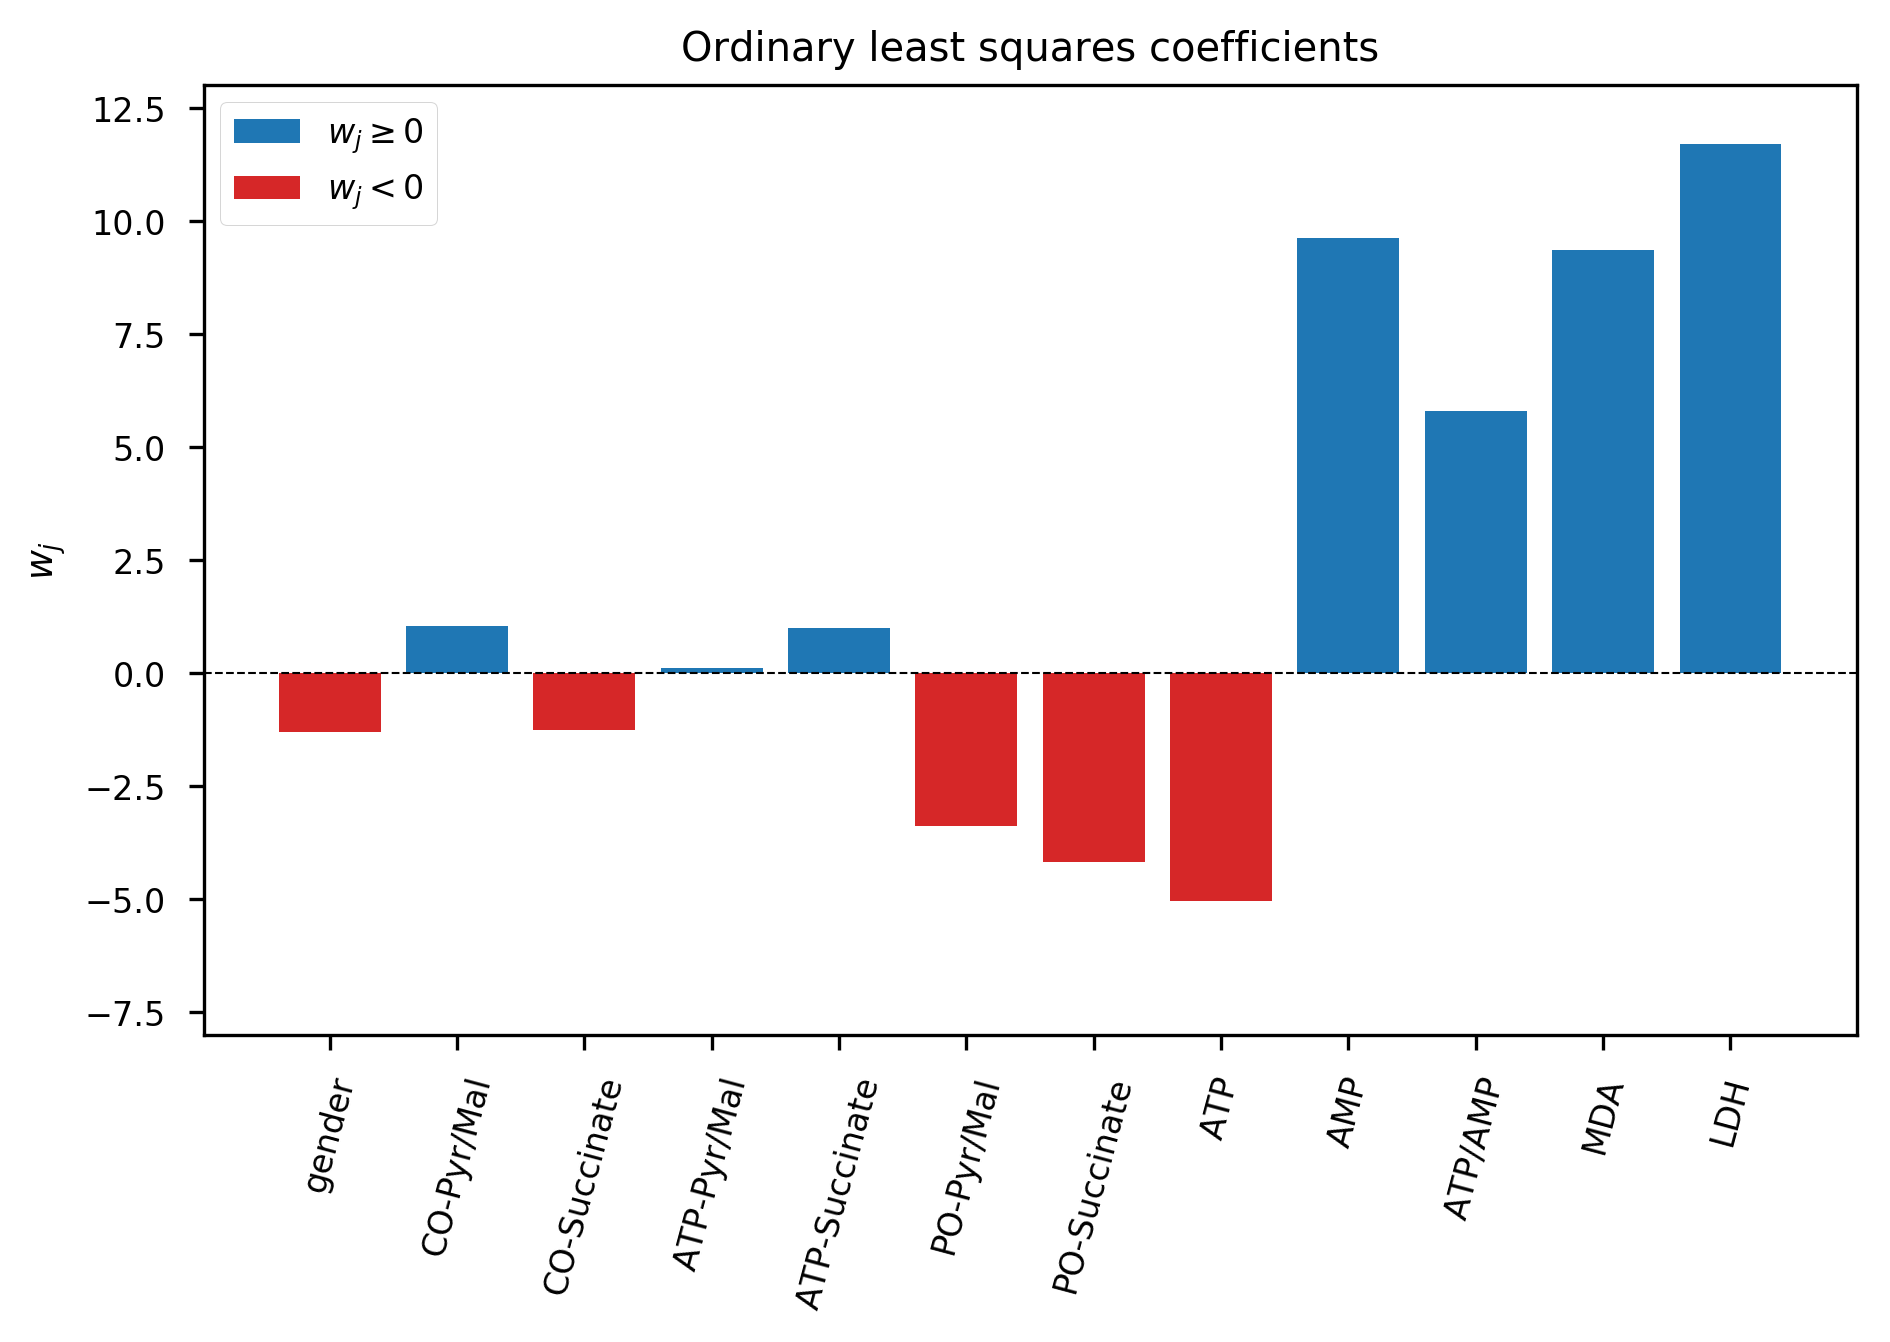
\includegraphics[width=0.8\textwidth]{part1/coefs_ols.png}
				\caption{A pictorial representation of the vector $\bm{\hat w}_{\text{OLS}}$ obtained fitting an OLS model on $74$ randomly selected training samples of $\mathcal{D}_{\text{aging}}$. Variables associated with positive (\ie directly proportional to the output) and a negative (\ie inversely proportional) weight are represented in blue and red, respectively.} \label{fig:coefs_ols}
		  \end{figure}
			As we can see, in order to achieve a predictive model, OLS can only spread the weights across all the input variables. Evaluating $\bm{\hat w}_{\text{OLS}}$ on the test set, this model has a Mean Absolute Error (\ac{MAE}) of $10.598$ years and explains the $74.29\%$ of the variance.

			This result looks promising, but we will see in the next sections if the use of various regularization penalties could help outperforming OLS.

%			We have already pointed out that learning predictive functions only by minimizing a loss function may lead to suboptimal solutions; therefore in the following sections we will explore pro and cons of using different penalties.

			\subsubsection{Ridge regression}
			In its original proposition, \textit{ridge regression}~\cite{hoerl1970ridge} is defined as a least squares problem penalized by the squared $\ell_2$-norm of the regression coefficients, see Equation~\eqref{eq:l2}.

			\begin{equation}\label{eq:l2}
				\mathcal{R}_{\mbox{$\ell_2$}}(\bm{w}) = \sum_{j=1}^d (w_j)^2 = \norm{\bm{w}}_2^2
			\end{equation}

			Therefore, the ridge regression minimization problem can be written as in Equation~\eqref{eq:ridge_regression}.

			\begin{equation} \label{eq:ridge_regression}
				\bm{\hat w}_{\ell_2} = \argmin_{\bm{w} \in \mathbb{R}^d} \frac{1}{n} \sum_{i=1}^n (\bm{x}_i^T\bm{w} - y_i)^2 + \lambda  \sum_{j=1}^d (w_j)^2 = \argmin_{\bm{w} \in \mathbb{R}^d} \frac{1}{n} \norm{X\bm{w} - \bm{y}}_2^2 + \lambda \norm{\bm{w}}_2^2
			\end{equation}

			This penalty leads to smooth solutions as it shrinks the coefficients toward zero, but it does not achieve a parsimonious representation, as it always keep all the variables in the model.
			The ridge regression problem of Equation~\eqref{eq:ridge_regression} is convex  and differentiable and a pictorial representation of its solution in a 2D case is depicted in Figure~\ref{fig:w_ridge}. The ridge coefficients $\bm{\hat w}_{\ell_2}$ can be estimated in closed-form as
			$$
				\bm{\hat w}_{\ell_2} = (X^TX + \lambda I)^{-1}X^T\bm{y}
			$$
			where $I$ is the $d \times d$ identity matrix. An estimate for the ridge coefficients can also be obtained with gradient descend-like optimization routines~\cite{boyd2004convex, sra2012optimization}.

			The regularization parameter $\lambda$ plays the fundamental role of balancing the trade-off between data adherence and smoothness of the solution.
			Penalizing the $\ell_2$-norm of the regression coefficients, their value is shrunk toward zero. This results in an increased robustness of the solution to the noise affecting training data.

			In case of multiple outputs, ridge regression can be easily extended to vector-valued regression problems, as in Equation~\eqref{eq:vvr_ridge}.
			\begin{equation} \label{eq:vvr_ridge}
				\begin{aligned}
					\hat W_{\text{F}}={} & \argmin_{W \in \mathbb{R}^{d \times k}} \frac{1}{n} \sum_{i=1}^n \sum_{t=1}^k (\bm{x}_i^T\bm{w}^t - y_i^t)^2  + \lambda \sum_{i=1}^n \sum_{t=1}^k |w_i^t|^2\\
					& =	\argmin_{W \in \mathbb{R}^{d \times k}} \frac{1}{n} \norm{XW - Y}_F^2 + \lambda \norm{W}_F^2
				\end{aligned}
			\end{equation}
			As already seen for vector-valued OLS, the Frobenius norm penalty does not induce any task coupling, hence solving the problem in Equation~\eqref{eq:vvr_ridge} still corresponds to individually solve $k$ regression tasks.

			As already pointed out for the OLS case, this method can be applied to binary classification problems by using the margin loss function of Equation~\eqref{eq:margin_square_loss}. Nevertheless, for $\ell_2$-norm penalized classification problems the use of the \textit{logistic loss} is usually preferred (see Section~\ref{sec:logistic_regression}).
%			ridge regression is successfully applied in countless and heterogeneous biological studies mainly involving regression problems.
%			For instance, in~\cite{kratsch2014} the authors propose a ridge regression-based method to estimate ancestral characters from phylogenetic trees, while in~\cite{bovelstad2007} ridge regression is used to perform survival prediction from gene expression data.
			%\todo{\begin{enumerate}
			%	% \item loss: square loss
			%	% \item penalties: l2
			%	% \item use in regression, classification
			%%	\item use cases
			%%	\item extension to multi-task and multi-class
			%\end{enumerate}}
			%Ridge regression can be extended to the case of multiple-output prediction for both vector-valued regression and multi-category classification problems.
			%In the first case,

			Let's see what happens when this method is applied to a real regression problem. For ease of comparison, we take into account the dataset $\mathcal{D}_{\text{aging}}$, introduced in Section~\ref{sec:ols}.
			Compared to OLS, ridge regression has the parameter $\lambda$ that must be fixed before fitting the model. In this example, we estimated the best $\lambda$ according to a standard grid-search cross-validation strategy~\cite{hastie2009elements}.
			This consists in fixing a range of ($30$) possible values for $\lambda$ (in a logarithmic scale from $10^{-3}$ to $10^2$) and
			pick the best value as the one achieving the lowest validation error, estimated via (5-fold) cross-validation.
			Therefore, once the best value for the regularization parameter ($\lambda = 20.43$) is fixed, the experimental setup used for OLS is preserved.
			The ridge coefficients $\bm{\hat w}_{\ell_2}$ are represented in Figure~\ref{fig:coefs_ridge}.
			\begin{figure}[!h]
				\centering
				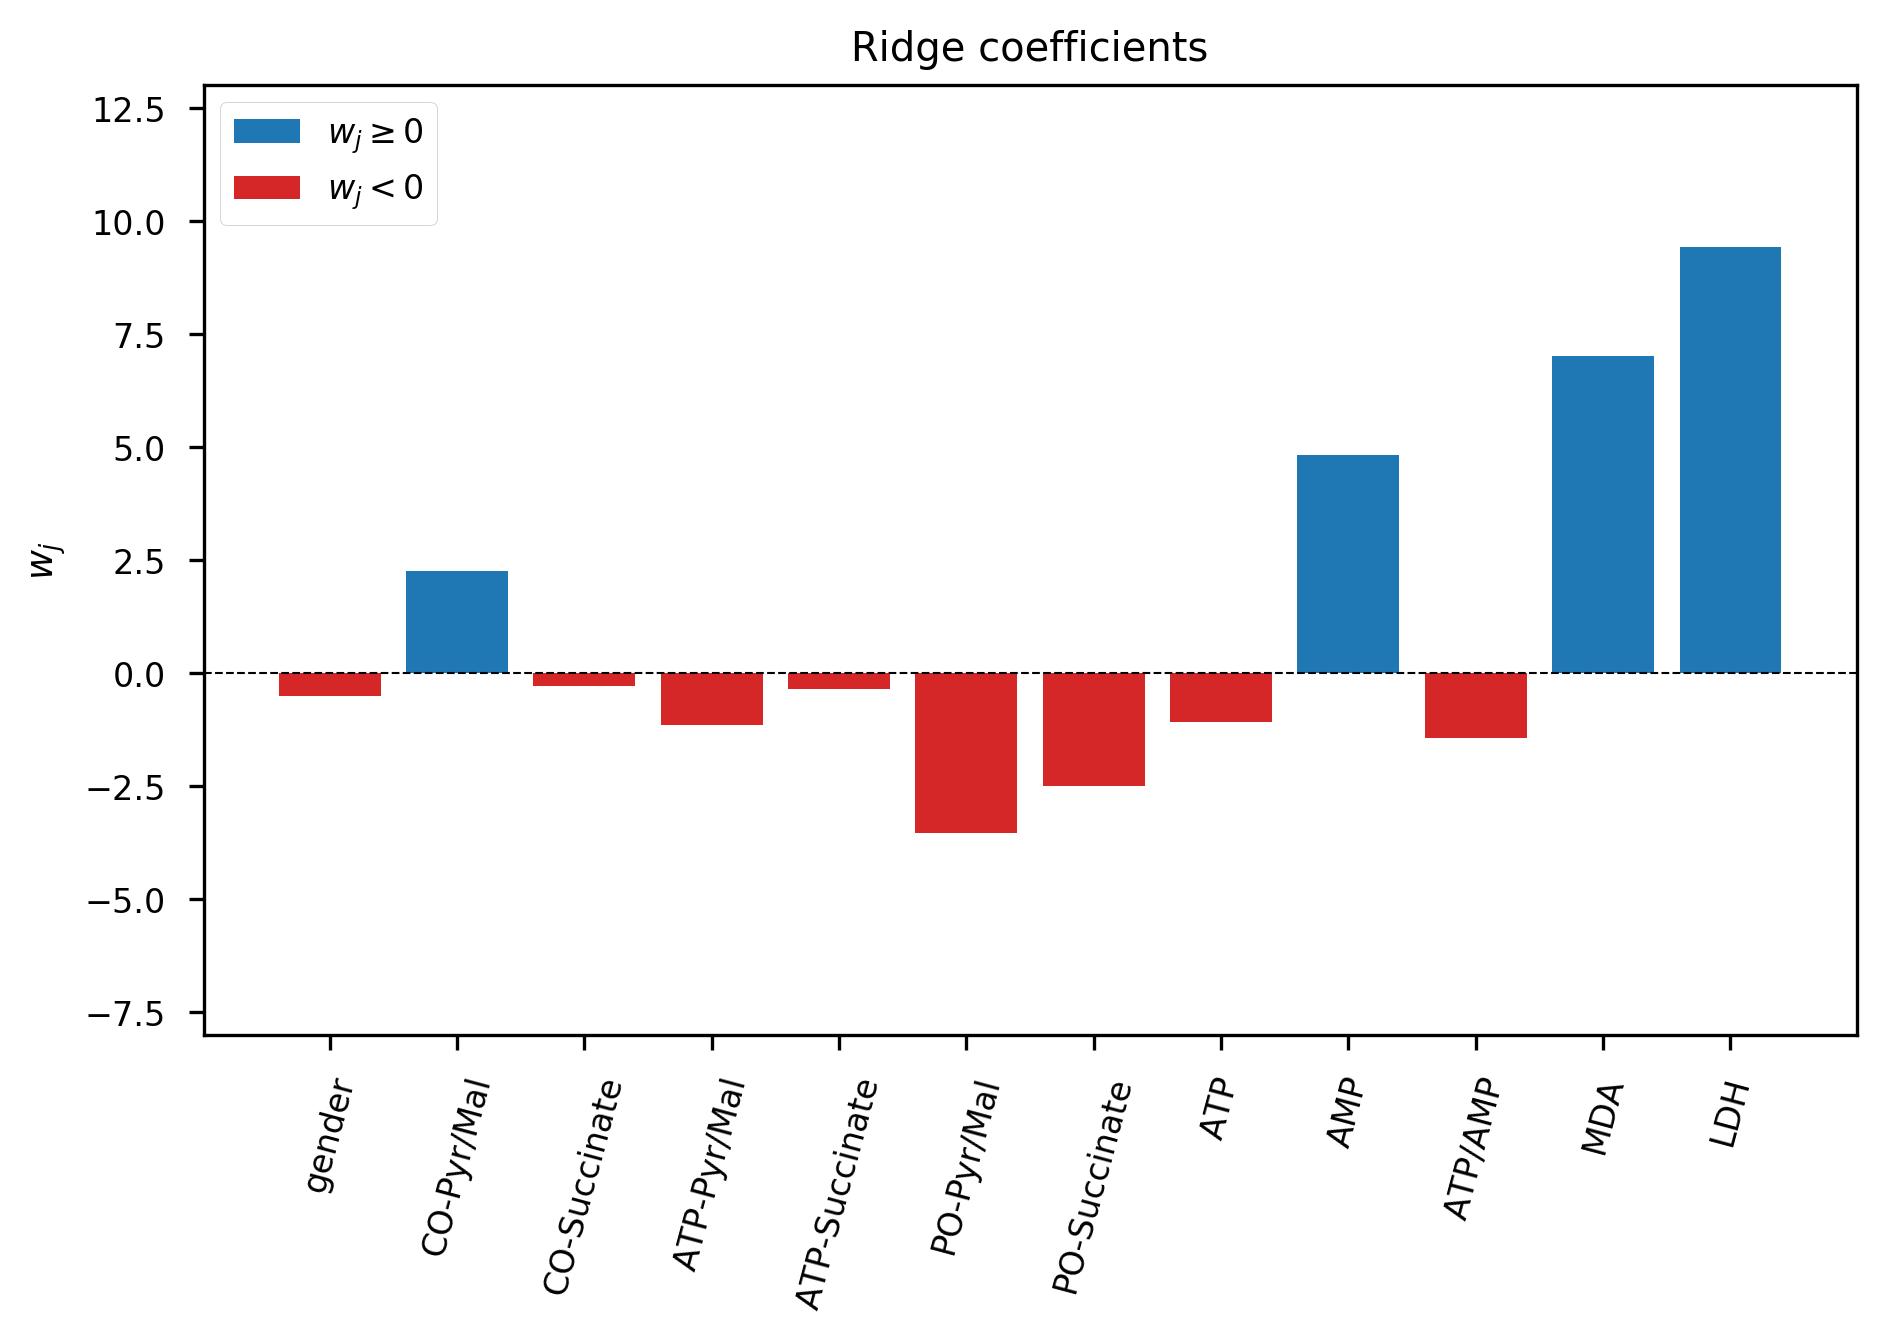
\includegraphics[width=0.8\textwidth]{part1/coefs_ridge.png}
				\caption{A pictorial representation of the vector $\bm{\hat w}_{\ell_2}$ obtained fitting a Ridge model on $74$ randomly selected training samples of $\mathcal{D}_{\text{aging}}$. Variables associated with positive (\ie directly proportional to the output) and a negative (\ie inversely proportional) weight are represented in blue and red, respectively.} \label{fig:coefs_ridge}
			\end{figure}
			Comparing Figure~\ref{fig:coefs_ridge} and Figure~\ref{fig:coefs_ols} we can see that the amplitude of the ridge regression coefficients is lower, in absolute value, several of them are very small, but none of them is exactly zero. This is the expected behavior of the $\ell_2$-norm penalty. Evaluating $\bm{\hat w}_{\ell_2}$ on the test set, this model has  $\text{MAE}=8.615$ years and explains the $81.19\%$ of the variance, outperforming OLS.

			\todo{add multitask}

			In deep learning literature, penalizing the regression coefficients with the $\ell_2$-norm is known as \textit{weight decay}~\cite{krogh1992simple}. Ridge regression can also be considered a form of  \textit{Tikhonov regularization}~\cite{tikhonov1963solution} and of \textit{regularization network}~\cite{evgeniou2000regularization}.


			%%%%%%%%%%%%%%%%%%%%%%%%%%%%%%%%%%%%%%%
			\subsubsection{Lasso}
			%Tibshirani, in its seminal paper~\cite{tibshirani1996regression}, introduced the use of the $\ell_1$-norm  Equation~\eqref{eq:lasso}, as sparisty-enforcing regularizer for least squares problems.
			%In the original Lasso paper, the sparisty-enforcing properties of the $\ell_1$-norm, Equation~\eqref{eq:lasso}, as regularizer for least squares problems is typically known as the Lasso.
			%Such penalty is among the most popular sparsity-enforcing regularization method.

			The Lasso~\cite{tibshirani1996regression} can be defined as a least square problem penalized by an $\ell_1$-norm, see Equation~\eqref{eq:lasso}.
			% In the Lasso, as in ridge regression (see Section~\ref{sec:ridge}), the data fidelity is measured by means of the square loss, while the $\ell_1$-norm, defined in Equation~\eqref{eq:lasso}, is used as regularization penalty.
			\begin{equation}\label{eq:lasso}
				\mathcal{R}_{\mbox{$\ell_1$}}(\bm{w}) = \sum_{j=1}^d |w_j| = |\bm{w}|_1
			\end{equation}
			Therefore, the Lasso minimization problem can be written as in Equation~\eqref{eq:lasso}.

			\begin{equation} \label{eq:lasso}
			\bm{\hat w}_{\ell_1} = \argmin_{\bm{w} \in \mathbb{R}^d} \frac{1}{n} \sum_{i=1}^n (\bm{x}_i^T\bm{w} - y_i)^2 + \lambda  \sum_{j=1}^d |w_j| = \argmin_{\bm{w} \in \mathbb{R}^d} \frac{1}{n} \norm{X\bm{w} - \bm{y}}_2^2 + \lambda |\bm{w}|_1
			\end{equation}


			The Lasso model is a popular  method for linear model fitting and embedded variable selection~\cite{guyon2003introduction} thanks to its desirable properties. At first, the $\ell_1$-norm of its regularization term enforces sparsity in the solution, hence producing compact and easily interpretable results. Secondly, the Lasso optimization problem is convex and, although non-differentiable, it is computationally feasible even in very high dimensional scenarios. Popular minimization algorithms for the Lasso problem are, for instance, the \textit{Fast Iterative Shrinkage-Thresholding Algorithm}  (\ac{FISTA})~\cite{beck2009fast} and the \textit{coordinate descent algorithm}~\cite{wu2008coordinate}. A pictorial representation of the Lasso solution can be seen in Figure~\ref{fig:w_lasso}.

			Let's see what happens when the Lasso model is applied to a real regression problem. Once again, for ease of comparison with OLS and ridge, we take into account the dataset $\mathcal{D}_{\text{aging}}$, introduced in Section~\ref{sec:ols}. The experimental setup in this case is identical to the one previously applied for ridge regression. The best value for the regularization parameter, chosen via grid-search cross-valudation, is $\lambda=1.27$. The Lasso coefficients $\bm{ \hat w}_{\ell_1}$ are represented in Figure~\ref{fig:coefs_lasso}.
			\begin{figure}[!h]
				\centering
				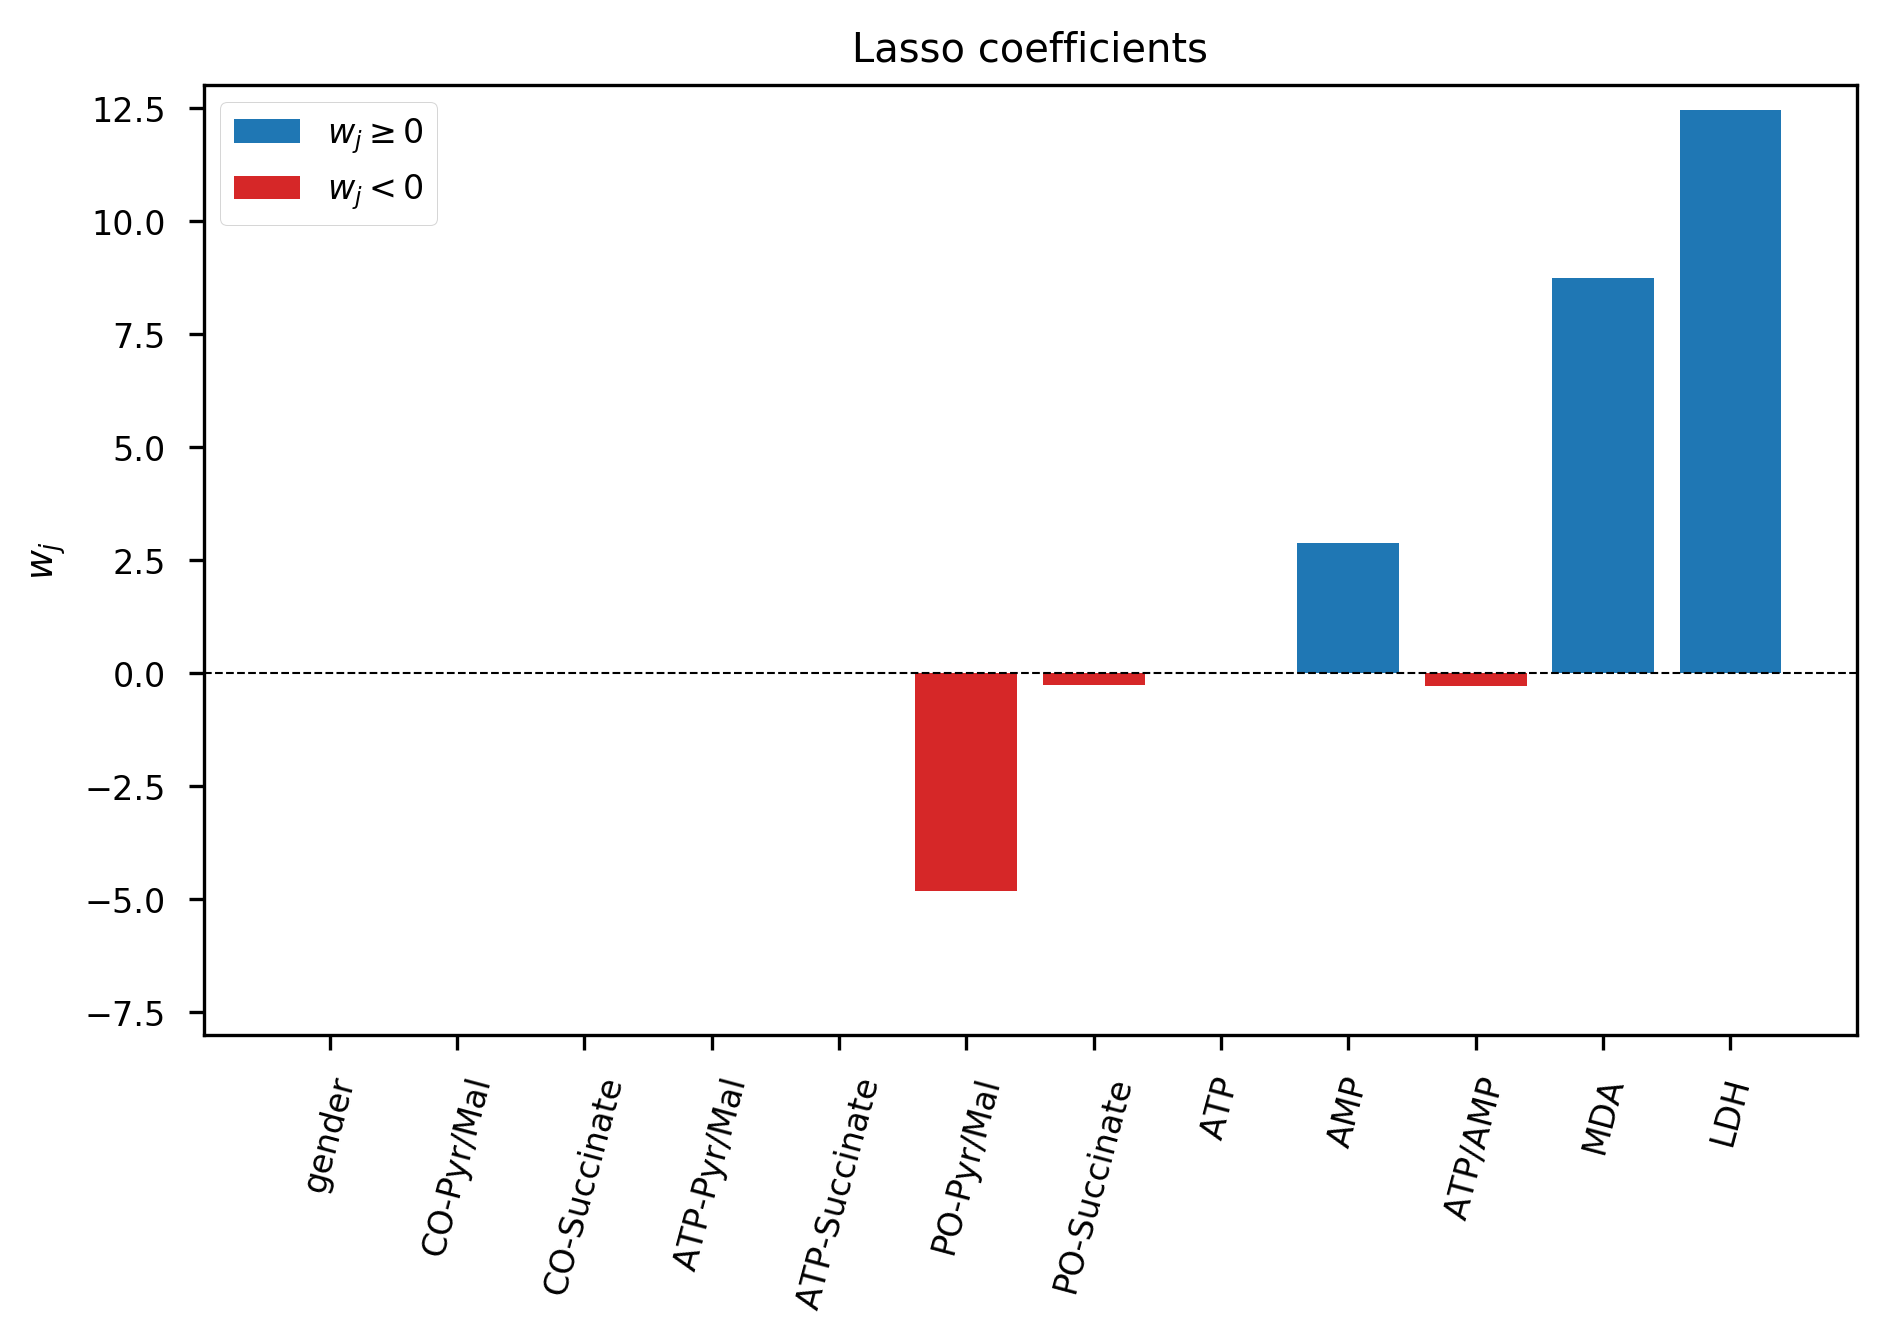
\includegraphics[width=0.8\textwidth]{part1/coefs_lasso.png}
				\caption{A pictorial representation of the vector $\bm{\hat w}_{\ell_1}$ obtained fitting a Ridge model on $74$ randomly selected training samples of $\mathcal{D}_{\text{aging}}$. Variables associated with positive (\ie directly proportional to the output) and a negative (\ie inversely proportional) weight are represented in blue and red, respectively.} \label{fig:coefs_lasso}
			\end{figure}
			Comparing $\bm{\hat w}_{\ell_1}$ with $\bm{\hat w}_{\ell_2}$ and $\bm{\hat w}_{\text{OLS}}$ (Figure~\ref{fig:coefs_lasso}, Figure~\ref{fig:coefs_ridge} and Figure~\ref{fig:coefs_ols}, respectively) we can observe that, for the first time, to only $6$ variables, out of $12$, a non-negative value is assigned. This is an example of the \textit{sparsity}-enforcing effect of the $\ell_1$-norm regularization penalty.
			The $6$ variables with nonzero weight can be considered as \textit{selected} for the prediction problem at hand.
			Evaluating $\bm{\hat w}_{\ell_1}$ on the test set, the Lasso has  $\text{MAE}=8.387$ years and explains the $81.51\%$ of the variance, slightly outperforming ridge.

			Originally proposed to solve regression problems, the Lasso can also be adopted in binary classification tasks; although, in this case, sparse Logistic regression (see Section~\eqref{sec:logistic_regression}) is often preferred~\cite{tong2009genome}.

			A popular application of the Lasso is to perform shrinkage and variable selection in survival analysis for Cox proportional hazard regression \cite{tang2017spike, gui2005penalized, tibshirani1997lasso} and additive risk models~\cite{ma2007additive}.
			Such $\ell_1$-penalized methods are extensively applied in literature to predict survival time from molecular data collected from patients affected by different kinds of tumor.

			%\todo{Add use cases: lu2011lasso, rakitsch2013lasso $\dots$}

			The Lasso can also be extended to vector-valued regression problems by using the mixed $L_{2,1}$-norm, defined in Equation~\eqref{eq:L21}, as regularization penalty~\cite{gramfort2012mixed}.

			\begin{equation}\label{eq:L21}
                \mathcal{R}_{L_{2,1}}(W)= \sum_{j=1}^d\sqrt{\Bigg(\sum_{t=1}^k |w_j^t|^2\Bigg)} = \norm{W}_{2,1}
			\end{equation}

			Therefore, the vector-valued regularization problem can be written as in Equation~\eqref{eq:multitask_lasso}
			\begin{equation} \label{eq:multitask_lasso}
			\begin{aligned}
			\hat W_{L_{2,1}}={} & \argmin_{W \in \mathbb{R}^{d \times k}} \frac{1}{n} \sum_{i=1}^n \sum_{t=1}^k (\bm{x}_i^T\bm{w}^t - y_i^t)^2 + \lambda  \sum_{j=1}^d \sqrt{\Bigg(\sum_{t=1}^k |w_j^t|^2\Bigg)} \\
			& =	\argmin_{W \in \mathbb{R}^{d \times k}} \frac{1}{n} \norm{XW - Y}_F^2 + \lambda ||W||_{2,1}
			\end{aligned}
			\end{equation}
			and it is known as Multi-task Lasso~\cite{lee2010adaptive}. Such norm enforces a row-structured sparsity in the regression weights, hence preserving the interpretability of the solution.

			When used for variable selection, the Lasso has two major drawbacks. First, in presence of groups of correlated variables, this method tends to select only one variable per group, ignoring the others. Secondly, the method cannot select more variables than the sample size~\cite{waldmann2013evaluation, de2009regularized}. In order to ameliorate this issues, several Lasso-inspired models were proposed~\cite{meinshausen2010stability, hoggart2008simultaneous, zou2006adaptive} (see Section~\ref{sec:other_sparsity}). In the next section we will describe one of the most famous and straightforward Lasso extensions: the Elastic-Net~\cite{zou2005regularization}.

			%Despite being a popular method
			%\todo{\begin{enumerate}
			%%	\item loss: square loss
			%%	\item penalties: l1
			%%	\item use in regression, classification
			%%	\item extension to multi-task and multi-class
			%%	\item use cases
			%\end{enumerate}}

			\subsubsection{Elastic-Net}
			The Elastic-Net~\cite{de2009elastic, zou2005regularization} method can be formulated as a least squares problem penalized by a convex combination of Lasso ($\ell_1$-norm) and ridge regression ($\ell_2$-norm) penalties, as in Equation~\eqref{eq:enet}.

			\begin{equation}\label{eq:enet}
				R_{\mbox{$\ell_1\ell_2$}}(\bm{w}) = \sum_{j=1}^d ((1-\alpha) |w_j| + \alpha w_j^2) = (1-\alpha)||\bm{w}||_1 + \alpha||\bm{w}||_2^2
			\end{equation}

			The combined presence of the $\ell_1$- and $\ell_2$-norms promote sparse solutions were groups of correlated variables can be simultaneously selected. It is easy to see that fitting the Elastic-Net model for $\alpha=1$ or $\alpha=0$ is equivalent to solve ridge or Lasso regression, respectively.

			The Elastic-Net method is successfully applied in several biomedical fields, including gene expression~\cite{jacob2015robust, de2009regularized}, genome-wide association studies~\cite{waldmann2013evaluation} and other molecular data~\cite{aben2016tandem, jacob2015robust}. In~\cite{csala2017sparse} the authors propose an iterative algorithm that exploits the variable selection capabilities of this method to estimate explanatory variables weights  in sparse redundancy analysis; such method is applied to explain the variability in gene expressions by epigenomic data (\ie methylation markers) collected from blood leukocytes of Marfan Syndrome patients.

			\begin{figure}[!h]
				\centering
				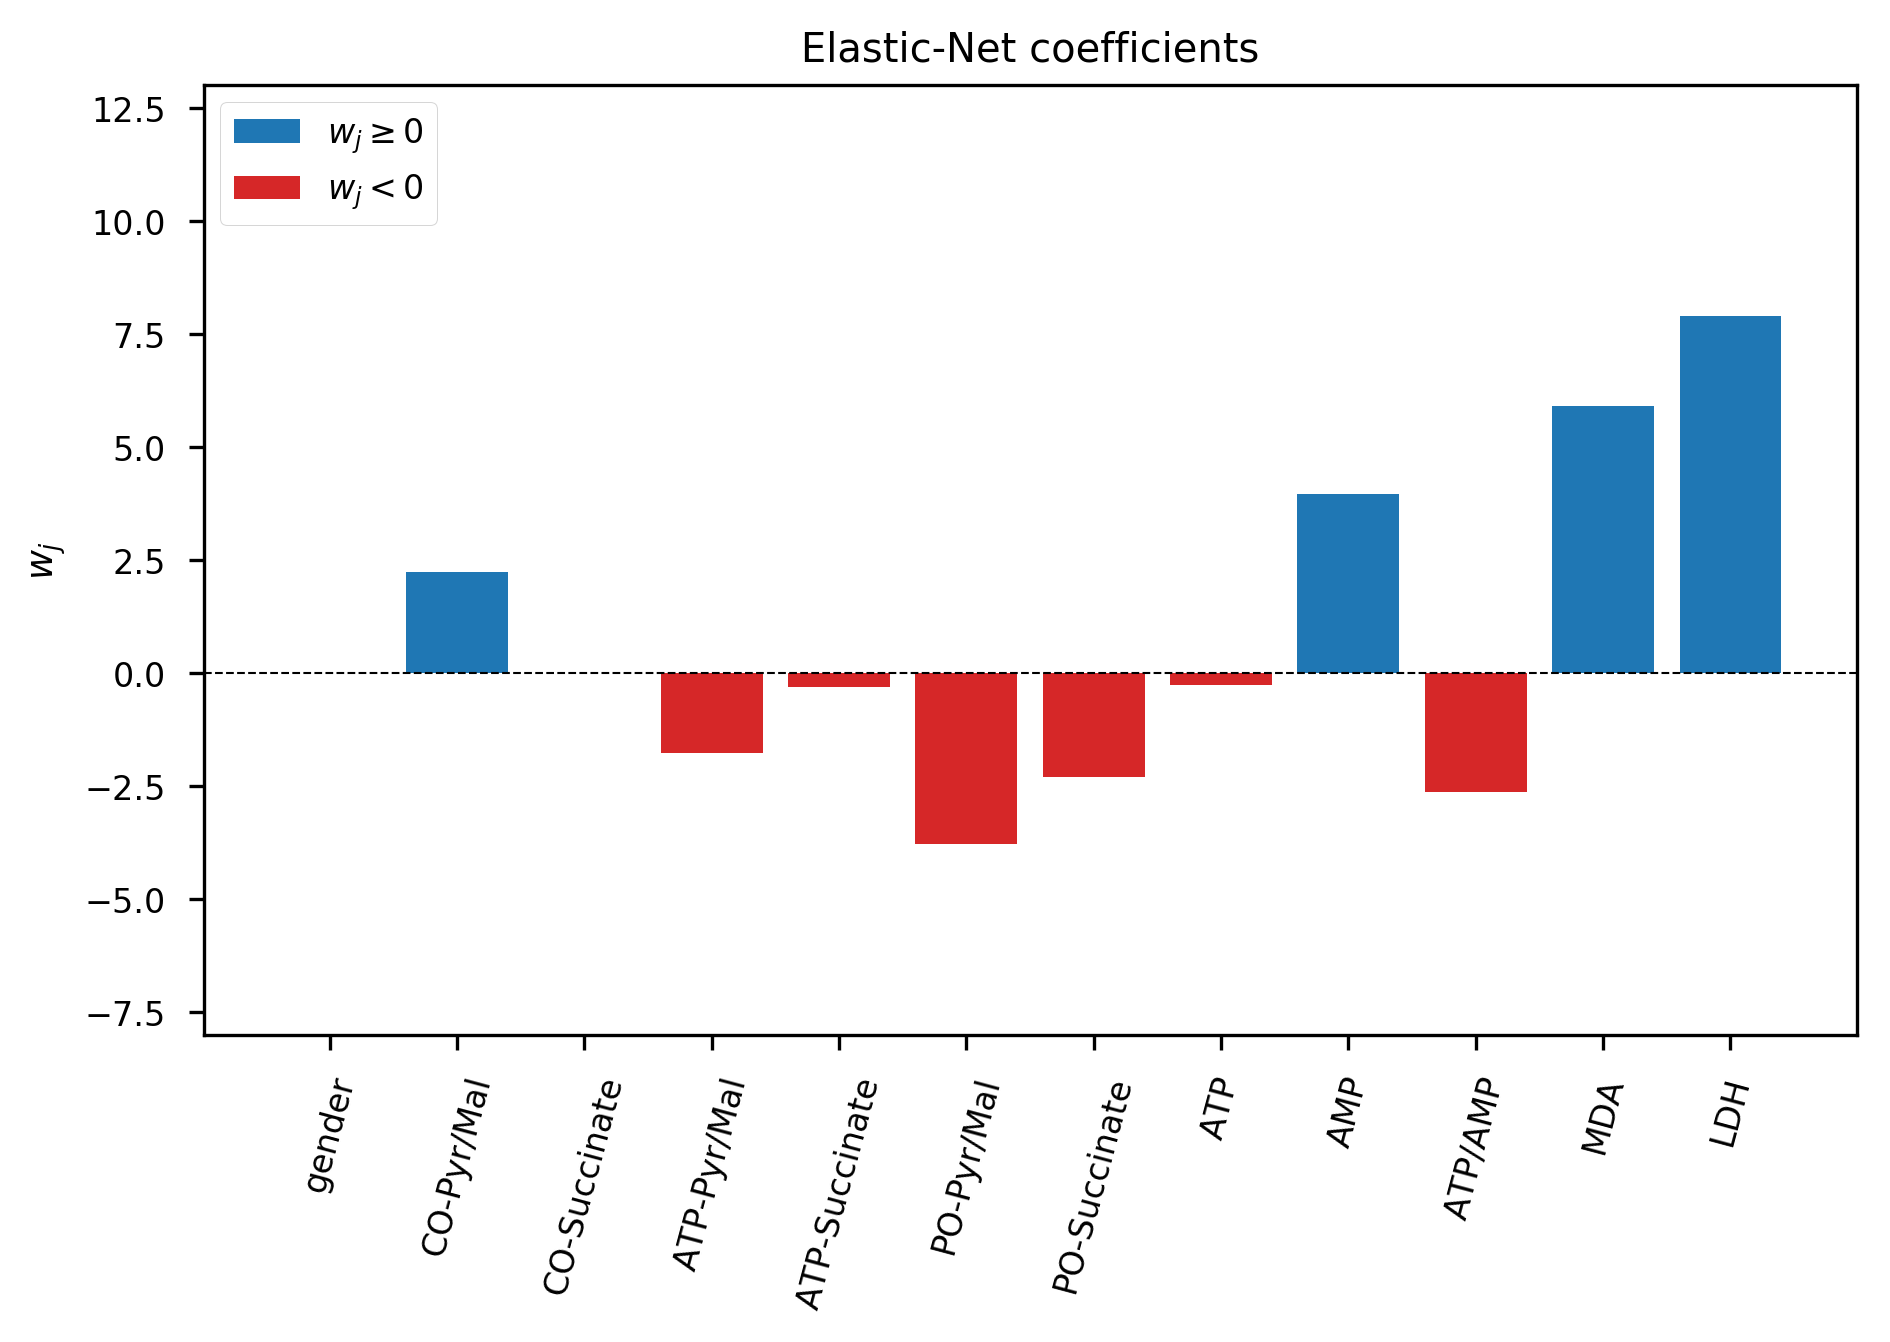
\includegraphics[width=0.8\textwidth]{part1/coefs_enet.png}
				\caption{A pictorial representation of the vector $\bm{\hat w}_{\ell_1\ell_2}$ obtained fitting a Ridge model on $74$ randomly selected training samples of $\mathcal{D}_{\text{aging}}$. Variables associated with positive (\ie directly proportional to the output) and a negative (\ie inversely proportional) weight are represented in blue and red, respectively.} \label{fig:coefs_enet}
		  \end{figure}

			This method can also be applied to vector-valued regression problems by simply replacing the $\ell_2$-norm with the Frobenius norm.
			\todo{As in $\dots$}~\cite{he2016novel}

			\begin{figure}[!h]
				\centering
				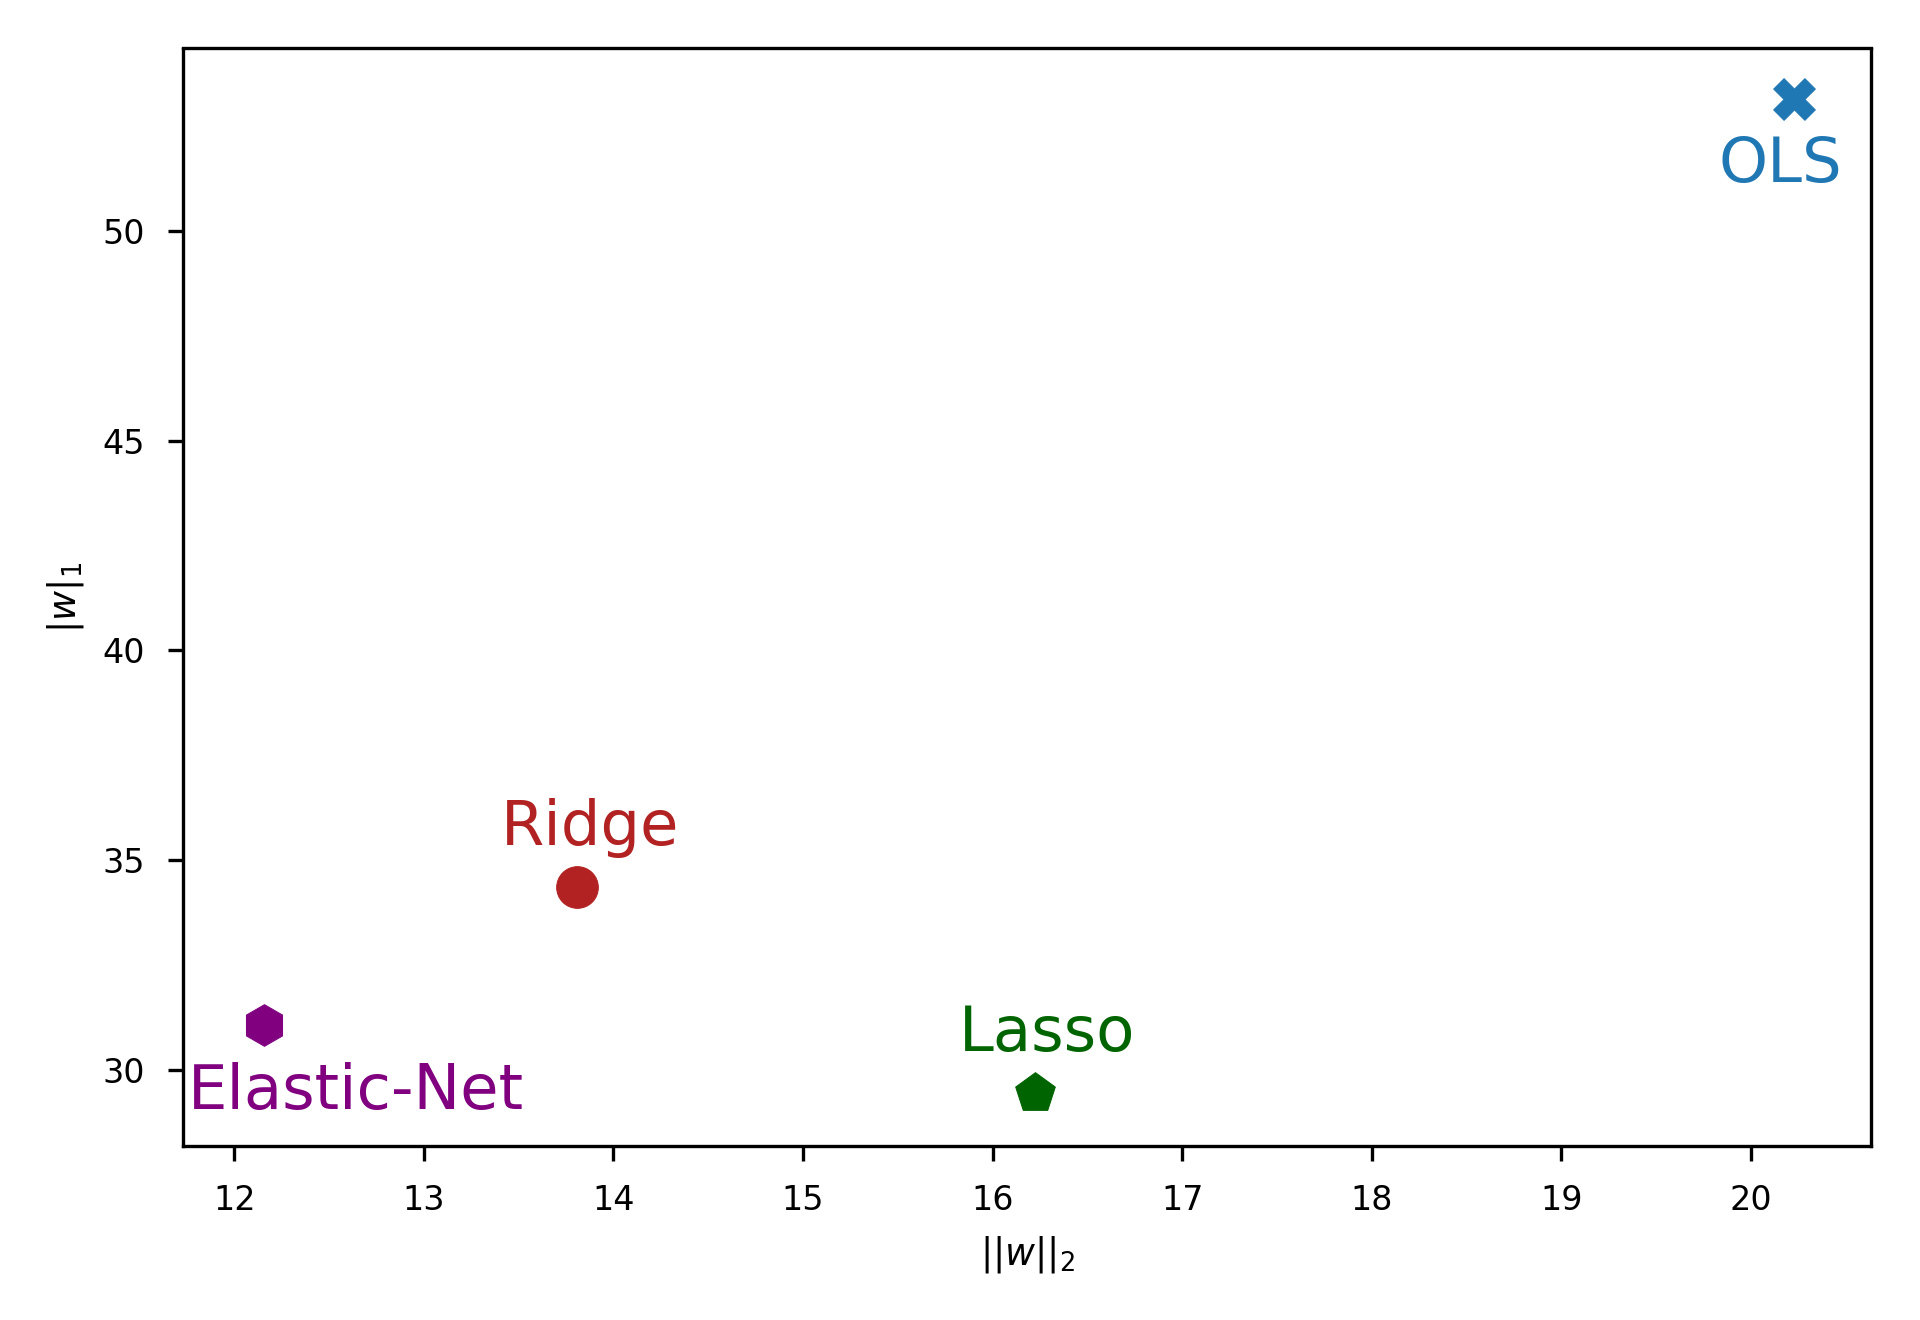
\includegraphics[width=0.8\textwidth]{part1/l1l2_norms_scatterplot.png}
				\caption{A comparison of the value of the $\ell_1$ and $\ell_2$ norms of the weights obtained by OLS, ridge, Lasso and Elastic-Net.} \label{fig:l1l2_norms_scatterplot}
		  \end{figure}

			\begin{figure}[h!]
				\centering
				\subfloat[]{%
					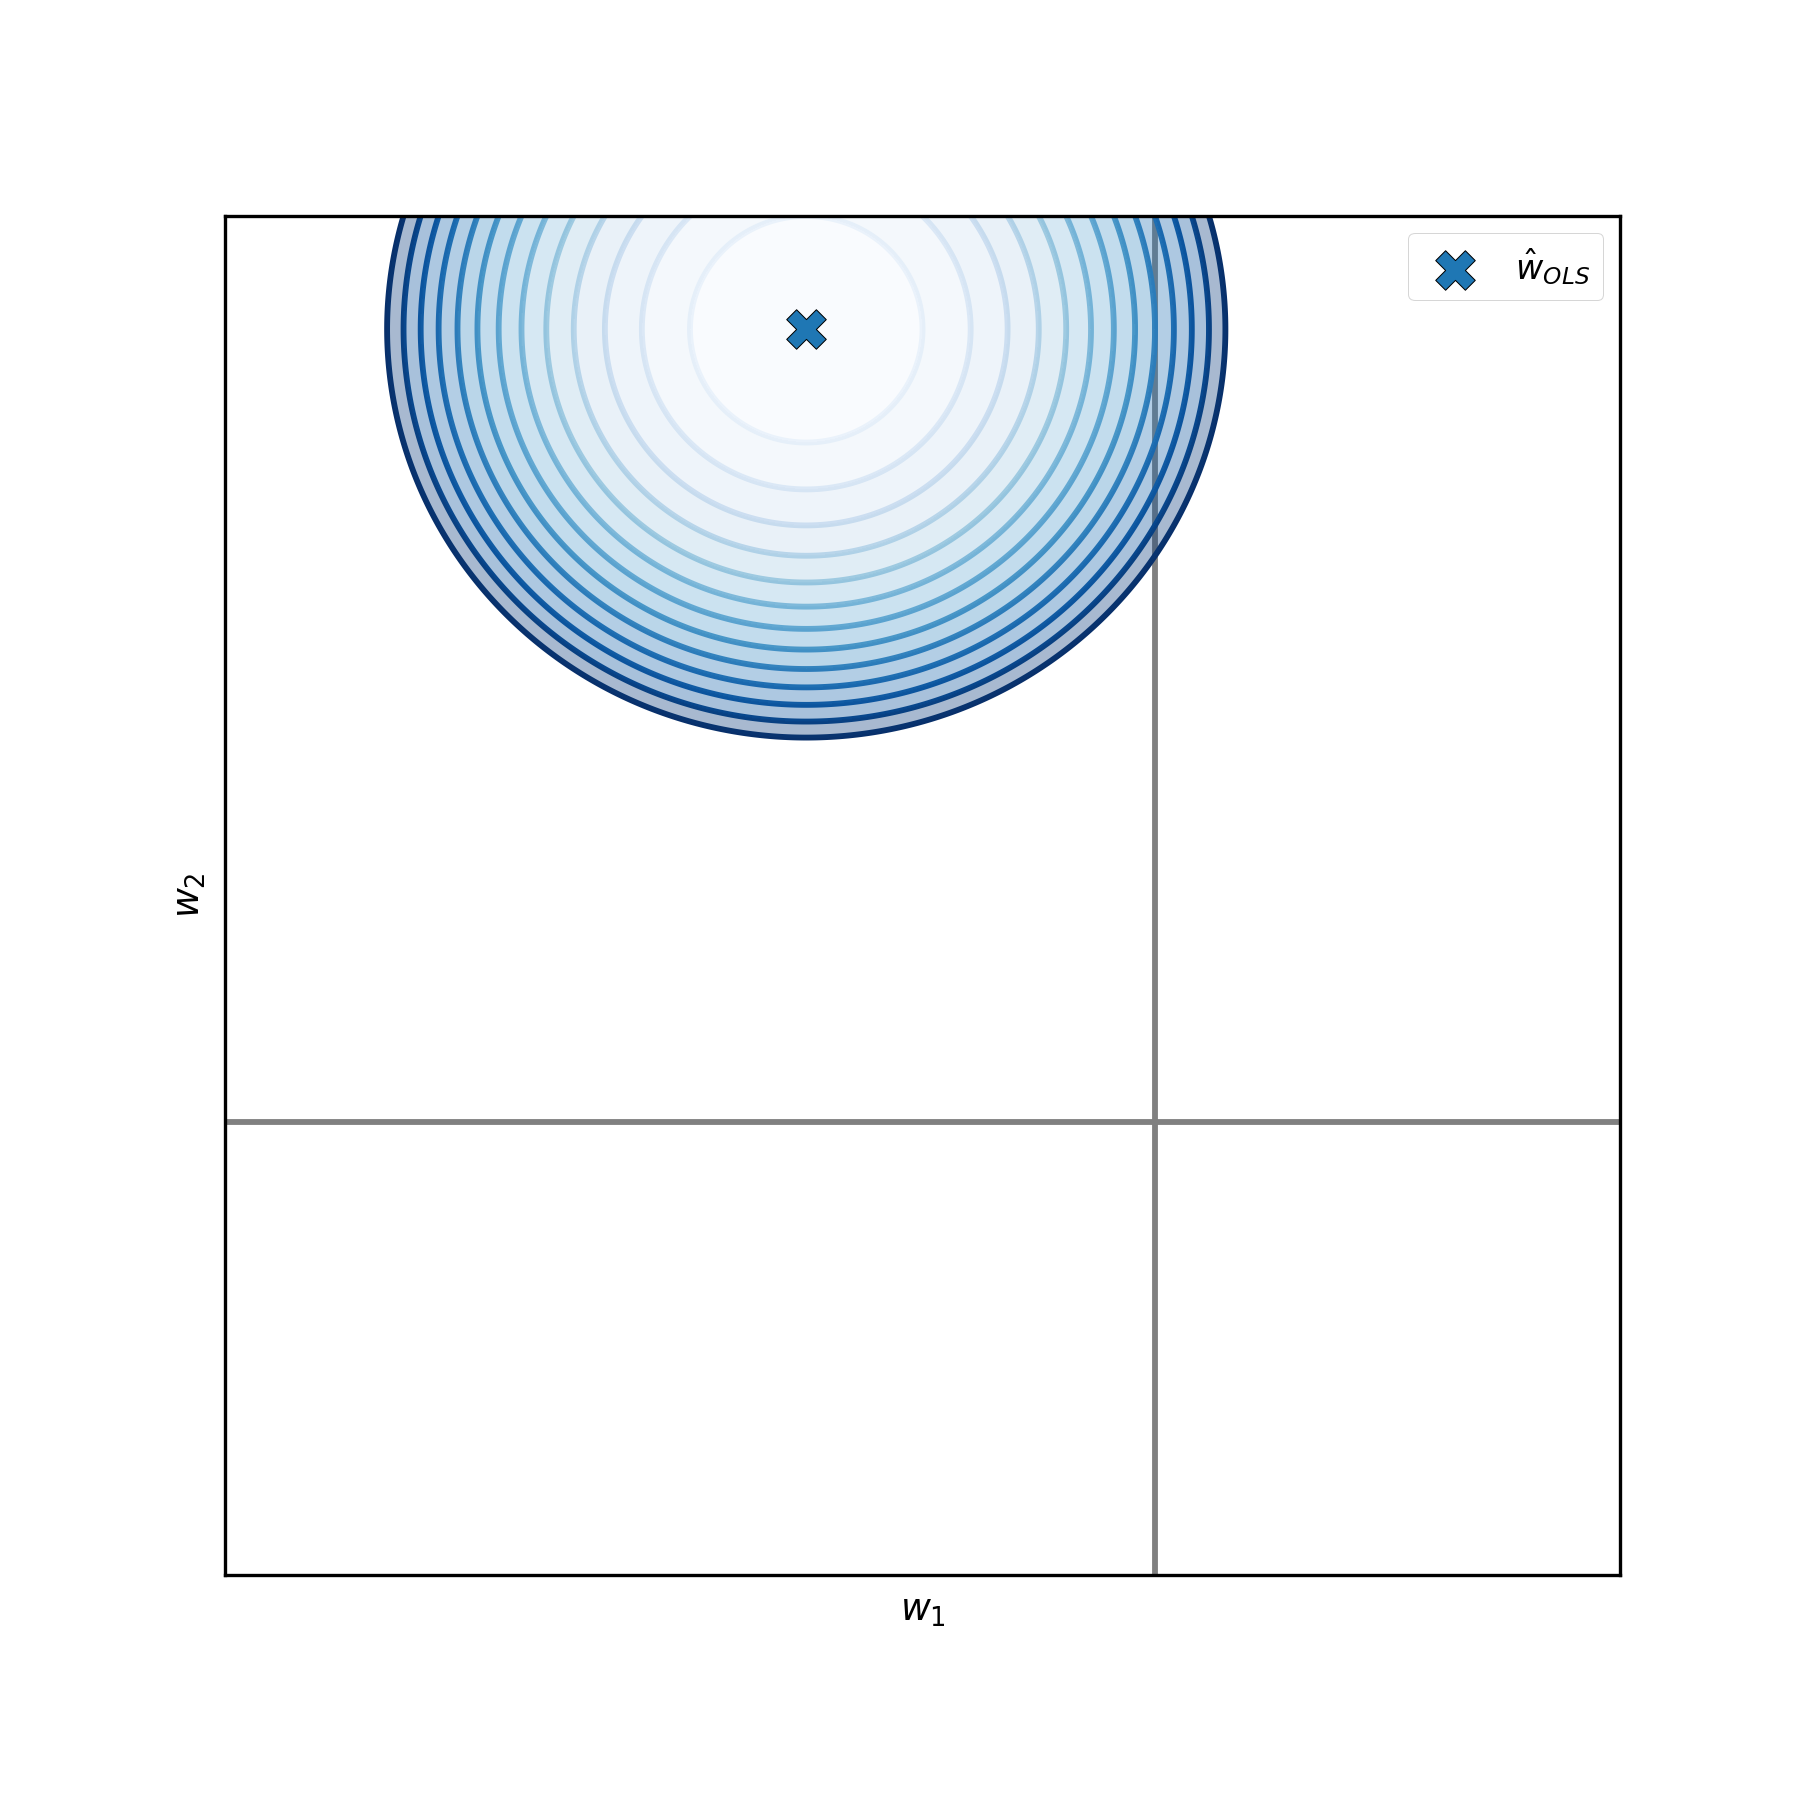
\includegraphics[width=0.5\textwidth]{part1/w_ols.png}
					\label{fig:w_ols}%
				}%
				%\hfill%
				\subfloat[]{%
					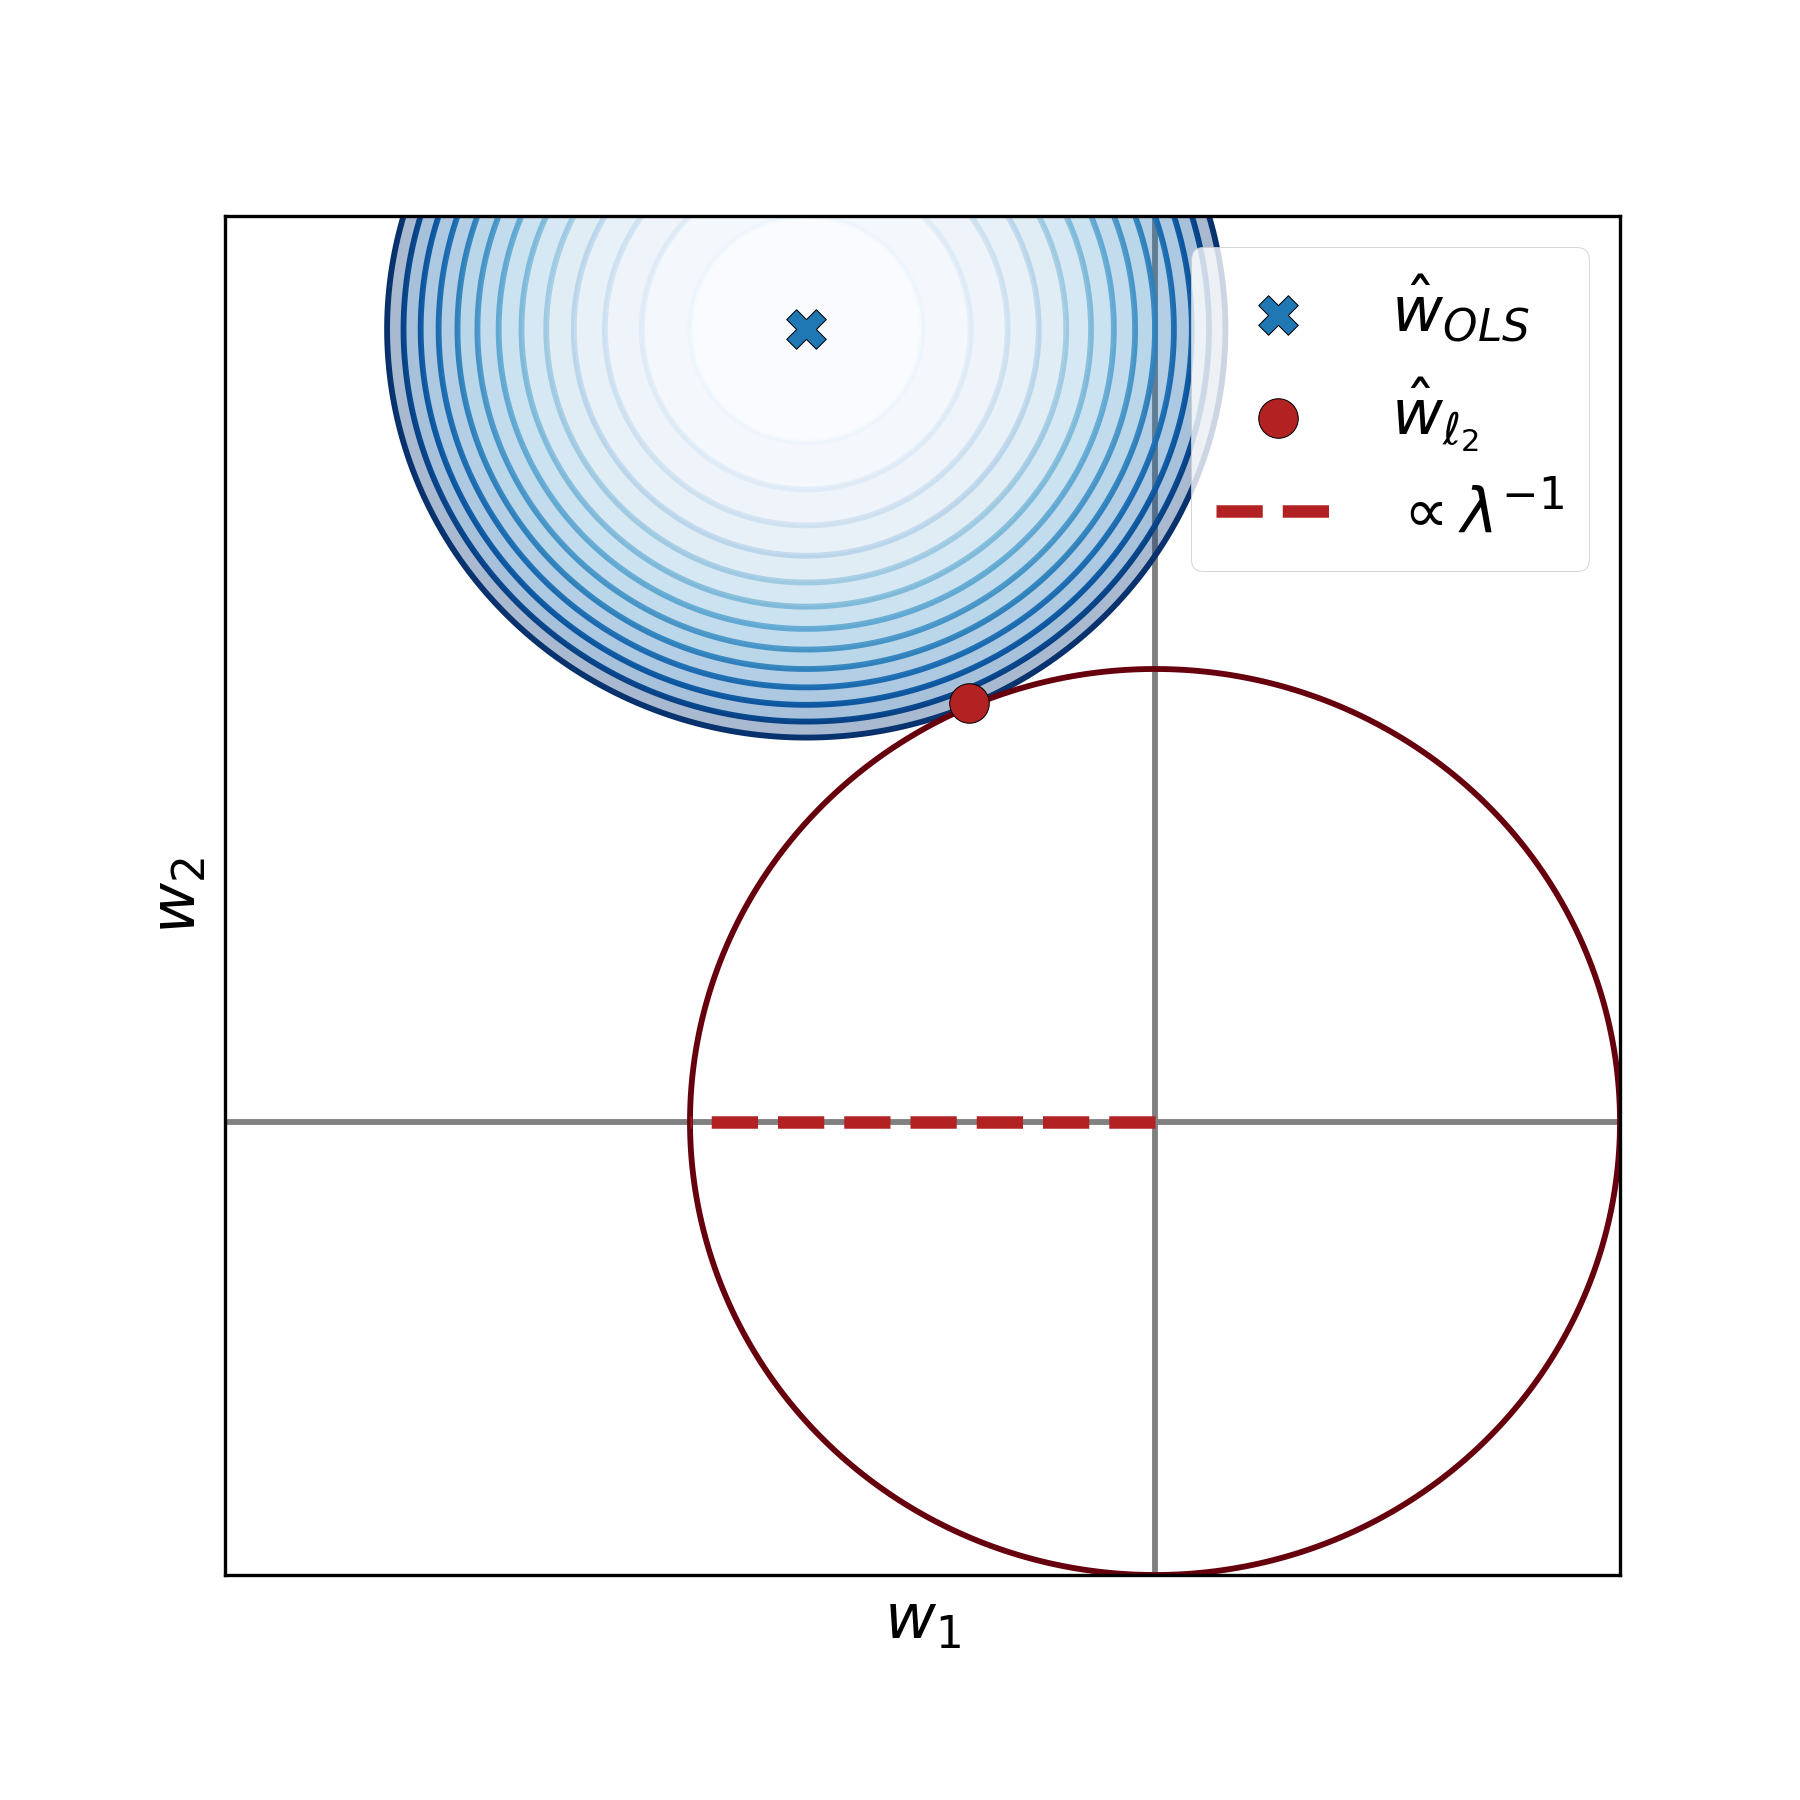
\includegraphics[width=0.5\textwidth]{part1/w_ridge.png}
					\label{fig:w_ridge}%
				}%
				\hfill%
				\subfloat[]{%
					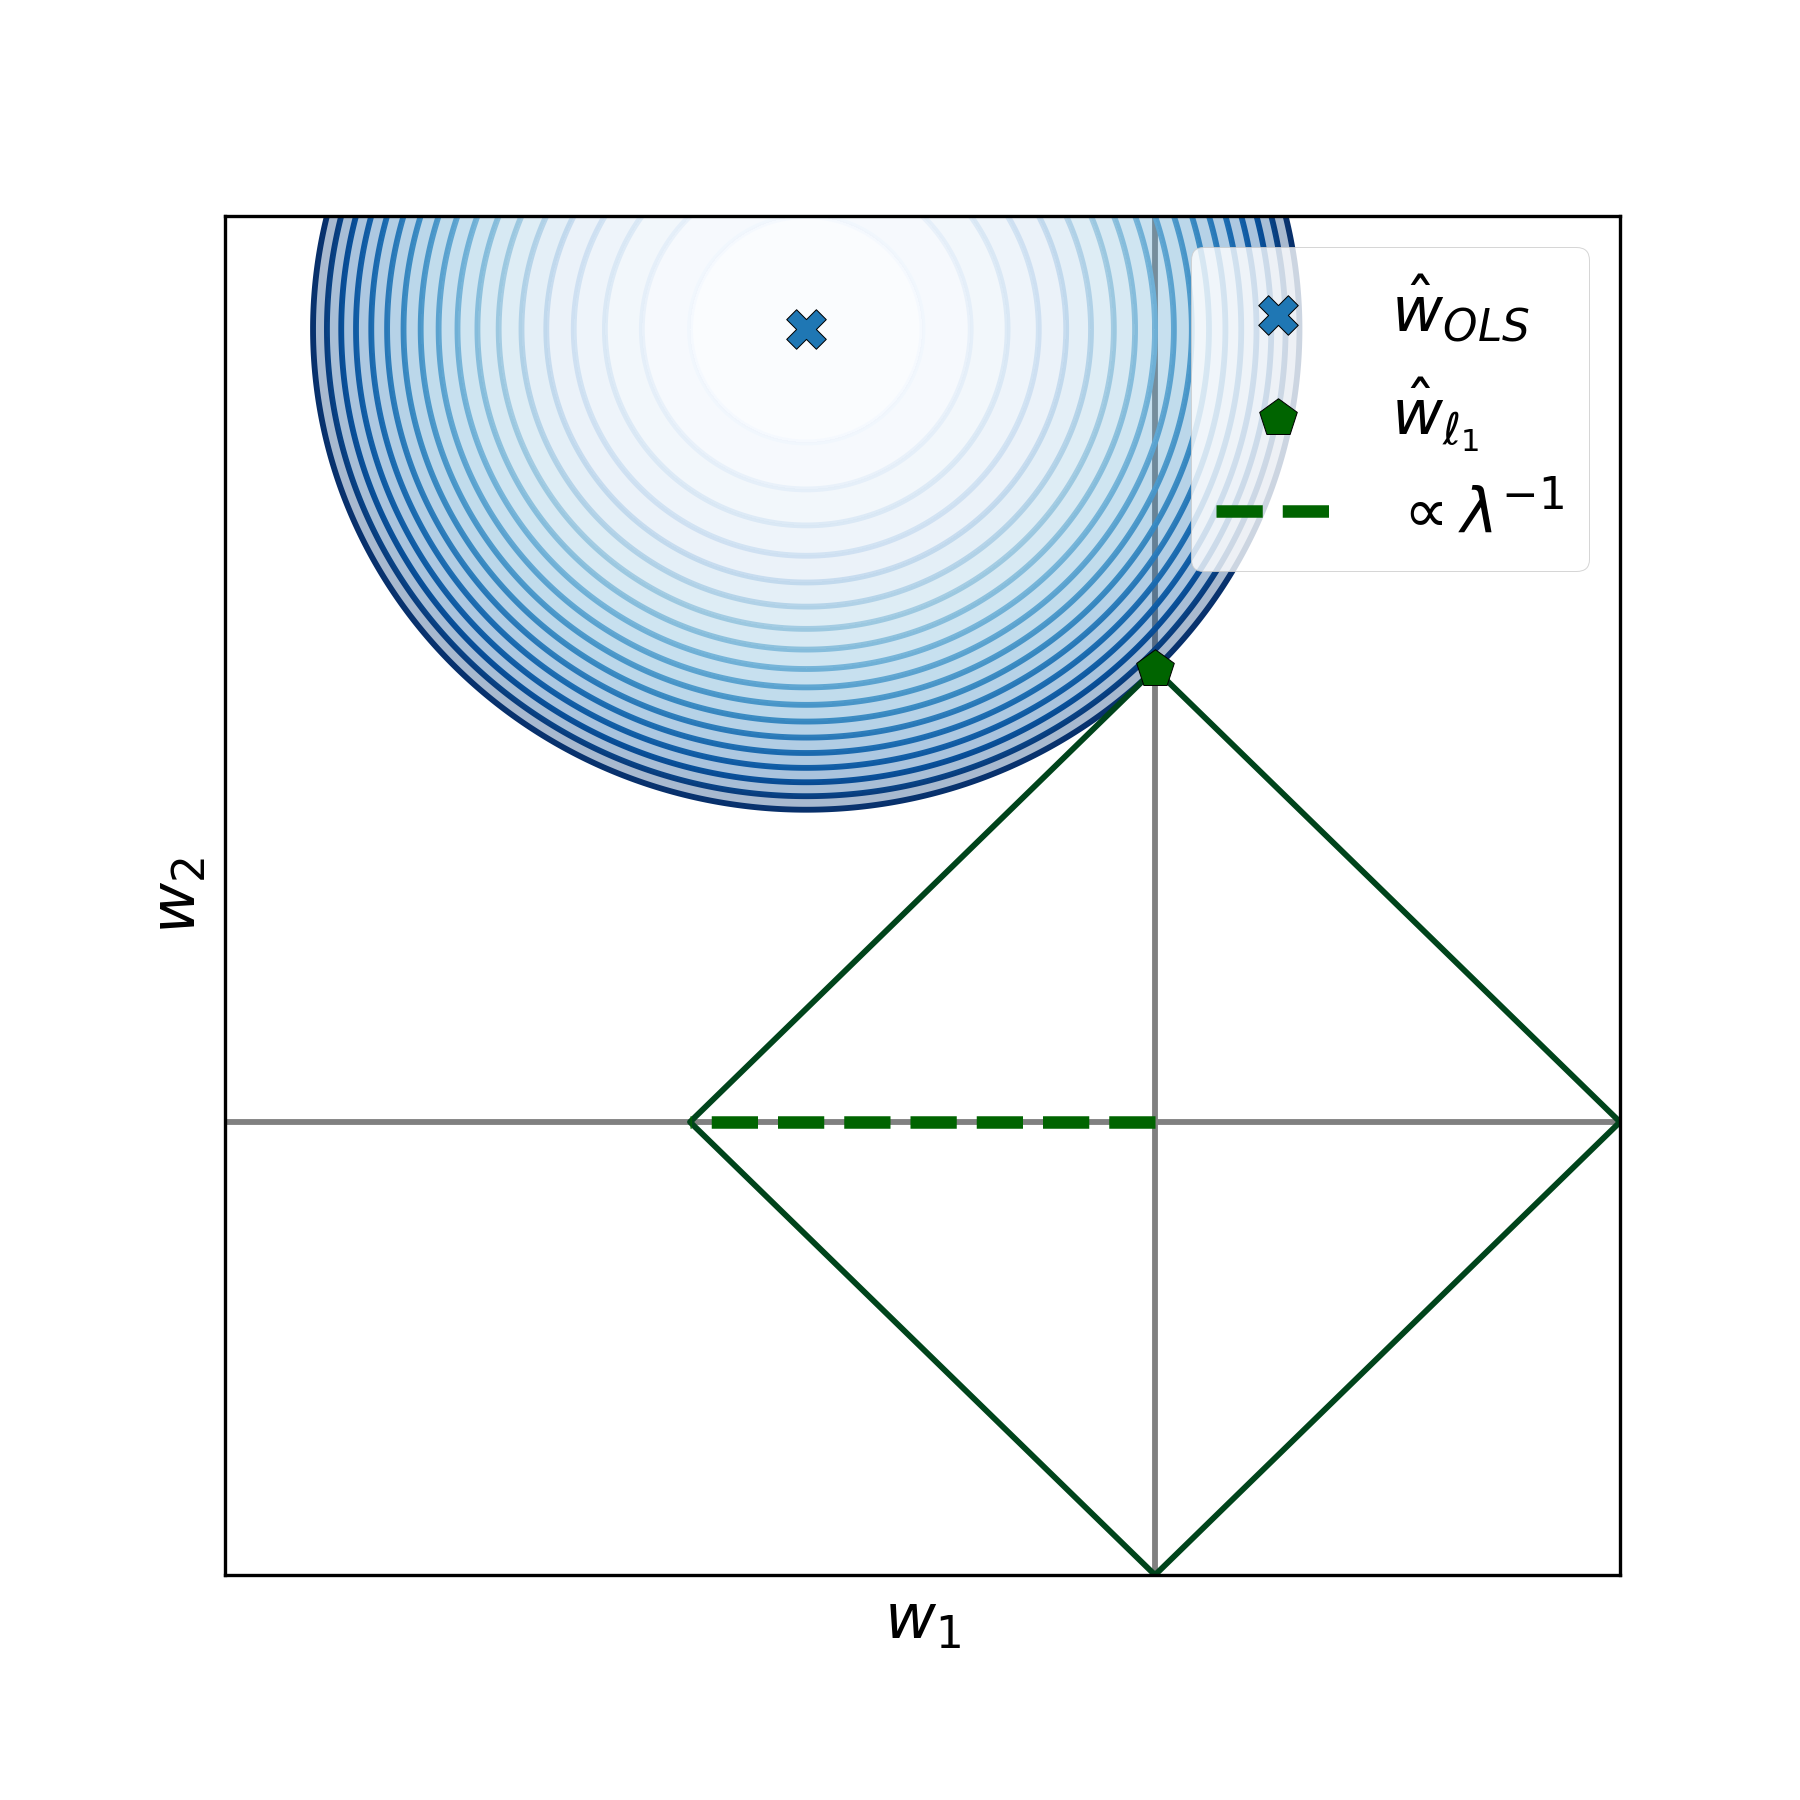
\includegraphics[width=0.5\textwidth]{part1/w_lasso.png}
					\label{fig:w_lasso}%
				}%
				%\hfill%
				\subfloat[]{%
					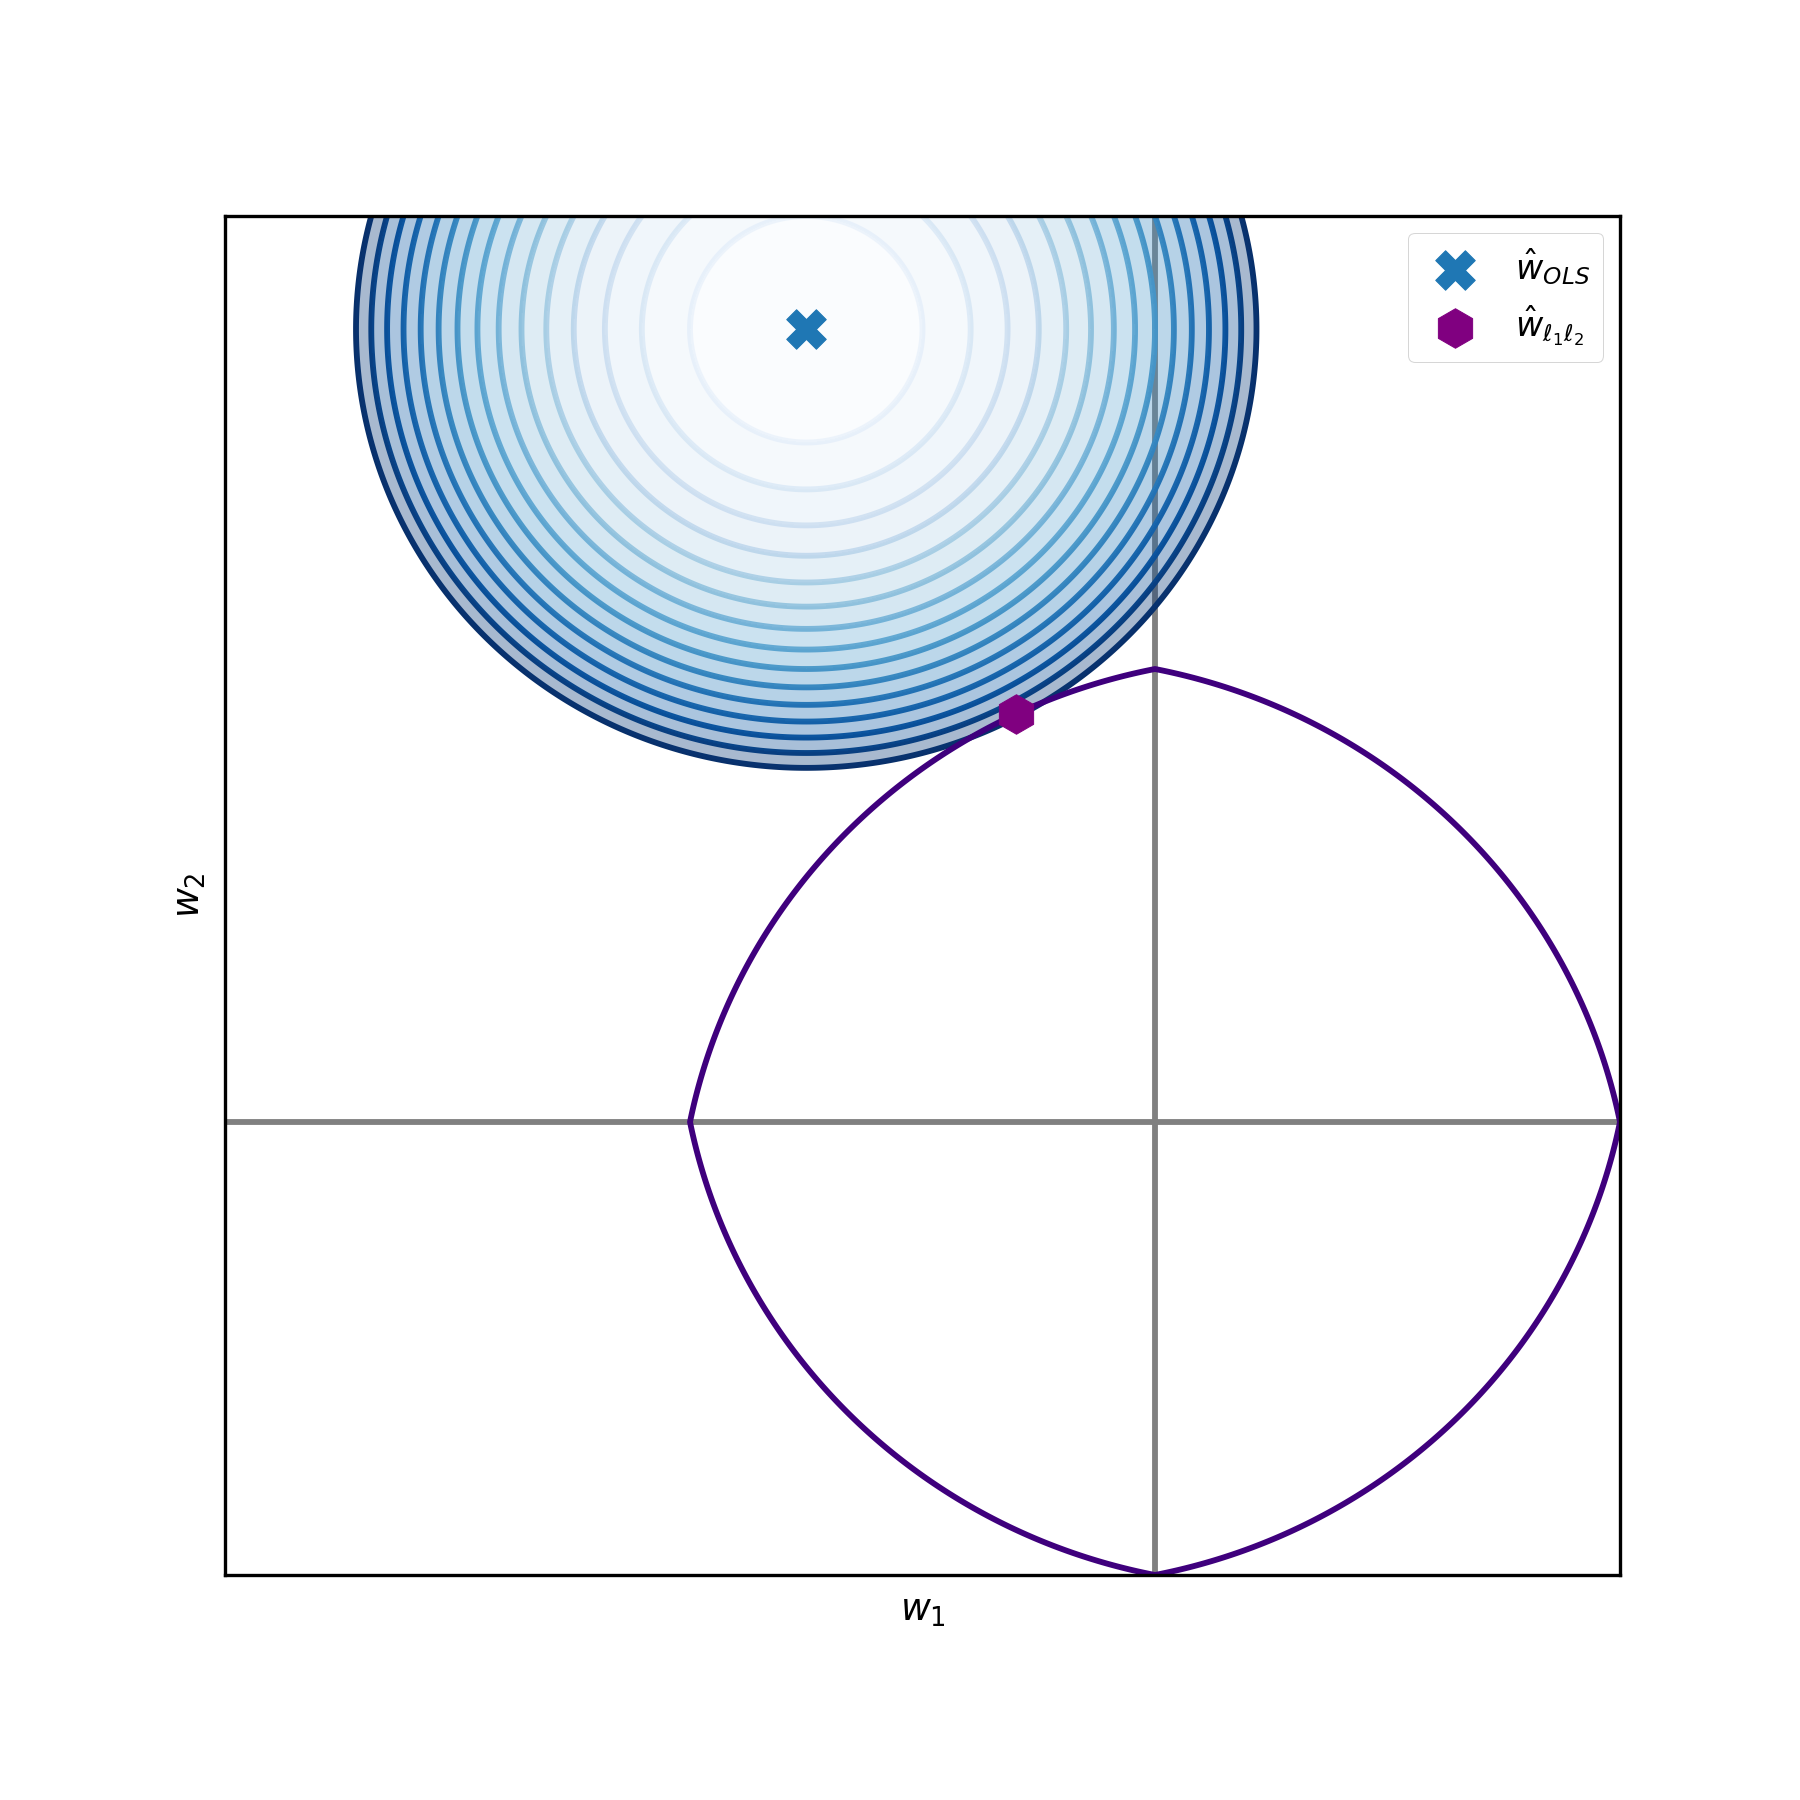
\includegraphics[width=0.5\textwidth]{part1/w_enet.png}
					\label{fig:w_enet}%
				}%
				\caption{Pictorial representation of the contour lines of the square loss in a 2D regression problem with various penalties: (a) ordinary least squares (no penalty), (b) ridge regression ($\ell_2$-norm penalty), (c) the Lasso ($\ell_1$-norm penalty) and finally (d) the Elastic-Net ($\ell_1$- and $\ell_2$-norm penalties).} \label{fig:square_loss_penalties}
			\end{figure}

			%%%%%%%%%%%%%%%%%%%%%%%%%%%%%%%%%%%%%%%
			\subsubsection{Other sparsity-inducing penalties}
			asd

			\begin{table}[htb]
				\centering
				\caption{Overview of the matrix norms used for vector-valued regression.}\label{tab:norms}
				\begin{tabular}{l|l|l}
					\toprule
					Matrix norm  & Notation         & Definition                      \\  \midrule
					Frobenius        & $\norm{A}_F$     & $\sqrt{\text{trace}(A^TA)}$     \\ [0.05cm]
					Nuclear          & $\norm{A}_*$     & $\text{trace}\sqrt{(A^TA)}$     \\ [0.05cm]
					Mixed $\text{L}_{2,1}$        & $\norm{A}_{2,1}$ & $\sum_{j}\norm{\bm{a}_j}_2$ \\ \bottomrule
				\end{tabular}
			\end{table}

			%%%%%%%%%%%%%%%%%%%%%%%%%%%%%%%%%%%%%%%
			\subsubsection{Logistic Regression} \label{sec:logistic_regression}
			\begin{enumerate}
				\item loss: logistic
				\item penalties: all the above apply
				\item use in classification
				\item extension to multiple-class: softmax regression
				\item use cases
			\end{enumerate}

			\todo{
			Some logistic regression works:
			\begin{enumerate}
				\item
			\end{enumerate}
			}

			Moreover, multi-class classification with Logistic regression is typically achieved by using either a \textit{One-vs-One} (OVO) or a \textit{One-vs-All} (AVA) approach~\todo{REF}.

			%%%%%%%%%%%%%%%%%%%%%%%%%%%%%%%%%%%%%%%
			\subsubsection{Support Vector Machines}
			\begin{enumerate}
				\item loss: hinge
				\item dual problem?
				\item penalties: l2 + l1
				\item use in classification and regression
				\item extension to multiple-class? (not sure)
				\item use cases
			\end{enumerate}



	    \subsection{Ensemble methods}
	    The key idea behind ensemble methods is to build a prediction model by aggregating a collection of multiple \textit{base learners} that are trained to solve the same problem~\citep{zhou2012ensemble}.

	    % FIXME
	    \textit{Bagging} is a common ensemble method that consists in fitting multiple models $f_b(\bm{x})$ for $b=1,\dots,B$ each one on a \textit{bootstrap} data set $\{X,\bm{y}\}_b$ obtained from the training set $\{X,\bm{y}\}$ by random sampling with replacement~\citep{hastie2009elements}. For each sample $\bm{x}_i$, the bagging estimate $\hat{f}(\bm{x}_i)$ is obtained by combining the predictions of the base learners $\hat{f}_b(\bm{x}_i)$. In particular, in case of classification tasks, the bagged model selects the most predicted class casting a vote among the $B$ base learners.

	    % FIXME
	    \textit{Boosting} is another popular ensemble method that, unlike bagging, performs predictions by sequentially fitting a collection of base learner that cast a weighted vote~\citep{hastie2009elements}. At each boosting step, the weight corresponding to samples that were misclassified at the previous iterations increases. Therefore, each successive classifier is somewhat forced to learn the relationships between input and output that were previously missed. From a theoretical standpoint, it would be possible to boost any learning machine, nevertheless boosting methods are mainly used with decision trees as base learners.


	    \subsubsection{Random Forests}
	    Decision trees are easily interpretable models that recursively partitions the training data into subsets, based on the test of a single feature value at each split (or node). At each iteration, the feature that yields the best split in terms of a pre-selected metric (Gini impurity, information gain or variance reduction) is chosen to create a new node. Decision trees tend to not perform well in practice, which led to the introduction of random forests in 2001~\cite{breiman2001random}.

	    Random forests are ensembles of decision trees, each grown on a bootstrap sample from the training data.
	    To increase robustness to noise and diversity among the trees, each node is split using the best split among a subset of features randomly chosen at that node.
	    The final prediction is made by aggregating the prediction of $m$ trees, either by a majority vote in the case of classification problems, or by averaging predictions in the case of regression problems.
	    Random forests are a {\it bagging} approach, which works on the assumption that the variance of individual decision trees can be reduced by averaging trees built on many uncorrelated subsamples.
	    By contrast, {\it boosted decision trees} are made by building an iterative collection of decision trees, trained by giving more importance to training examples that were incorrectly classified by the previous trees. \todo{Add use cases for boosted decision trees. $\dots$}

	    Random forests can provide several measures of {\it feature importance}, computed by looking at the increase in prediction error % (mean decrease in accuracy; mean decrease in node impurity)
	    when data for a feature is permuted while all other features remain unchanged. Feature selection based on random forests if most often performed using one of these measures. However, several techniques for applying regularization to random forests have been proposed. These techniques broadly fall under two categories: (1) cost-complexity pruning, which consists in limiting tree depth, resulting in less complex models~\cite{ishwaran2008random,kulkarni2012pruning}; and (2) Gini index penalization~\cite{deng2013gene, liu2014learning}. In addition,~\cite{joly2012ell1} proposed using an $\ell_1$-norm  to reduce the space-complexity of random forests.

	    Random forests naturally handle both numerical and categorical variables, multiple scales, and non-linearities. They also require little parameter tuning. This makes them popular for the analysis of diverse types of biological data, such as gene expression, GWAS data or mass spectrometry~\cite{qi2012random}. Unfortunately, in practice feature selection schemes that rely on them tend to be very unstable~\cite{kursa2014robustness}.

	    \subsubsection{Gradient Boosting}
	    \textit{Gradient boosting}~\citep{friedman2001greedy}  is one of the most widely applied boosting methods in biological problems.
	    %This technique iteratively combines the predictions obtained by several base learners, such as decision trees, into a single model.
	    The key idea behind gradient boosting is that, under some general hypothesis on the cost function, boosting can be seen as an iterative gradient method for numerical optimization.
	    %In particular, in GB at each boosting step a new base learner is fitted on the residuals obtained at the previous boosting iteration.
	    Gradient boosting has several desirable properties~\citep{mayr2014evolution}, such as its capability to learn nonlinear input/output relationship, its ability to embed a feature importance measure (as random forests~\citep{hastie2009elements}) and its stability in case of high-dimensional data~\citep{buehlmann2006boosting}.

	    %The consistency of GB in high-dimensional problems was demonstrated in.

	    As for any learning machine, boosting methods may suffer of overfitting. The main regularization parameter to control is the number of boosting iterations $M$, \ie the number of base learners, fitted on the training data. This is typically optimized by cross-validated grid-search, or by information criteria-based heuristics~\citep{tutz2006generalized, tutz2007boosting} (see Section~\ref{subsec:model_selection}).

	    Regularization in gradient boosting can also be controlled by shrinking the contribution of each base learner by a constant $0<\nu<1$ that controls the learning rate of the boosting procedure~\citep{hastie2009elements}. In order to achieve comparable predictive power, smaller values of $\nu$ imply larger number of $M$, so there is a tradeoff between them.
	    As usually the base learners are decision trees, another important parameter to tune is their maximum depth~\citep{hastie2009elements}.

	    In a recent paper~\citep{lusa2015boosting}, the authors show that in high-dimensional balanced binary classification problems, if the base learner is likely to overfit the training data, the use of \textit{Stochastic gradient boosting}~\citep{friedman2002stochastic} is preferable. The latter is a modified version of the original method, where each base learner is fitted on a random extraction without resubmission of a fraction $\eta$ of the training data, where $\eta$ is de-facto a regularization parameter to choose.

	    Approaches based on gradient boosting classification are used to detect \textit{de novo} mutations showing an improved specificity and sensitivity with respect to state-of-the-art methods~\citep{liu2014gradient}.
	    When combined with stability selection~\citep{meinshausen2010stability}, gradient boosting has demonstrated to be a very resourceful method for variable selection, leading to an effective control of the false discovery rate. This strategy was followed to associate overall survival with single-nucleotide polymorphisms of patients affected by cutaneous melanoma~\citep{he2016component} and to detect differentially expressed amino acid pathways in autism spectrum disorder patients~\citep{hofner2015controlling}.

	    \todo{consider adding boosting method for cox models...}



	%%



	    \subsection{Deep learning}
	    % I shall not forget that this is Regularization in bio studies, there are plenty of ML in bio studies out there
	    Deep Learning (DL) methods are a broad class of machine learning techniques that, starting from raw data, aim at learning a suitable feature representation (see Section~\ref{sec:unsupervised}) and a prediction function, at the same time~\cite{lecun2015deep}. DL methods can be seen as an extension of classical Neural Networks, where the final prediction is achieved by composing several layers of non-linear transformations.
	    %The intuition behind DL method is that, starting from raw data, their multi-layer architecture can achieve representations at a more abstract level, capable of achieving high performance in prediction tasks.
	    DL architectures can be devised to tackle binary/multi-category classification~\cite{angermueller2016deep, leung2014deep} as well as single/multiple-output regression~\cite{Chen2016GeneEI, ma2015deep} tasks.
	    %\todo{microarray gene xpression multi-task regression }

	    Many methods fall in this class~\cite{lecun2015deep}, in order to understand them in general, we sketch here the main ideas behind the most basic one: the Multi-Layer Perceptron (MLP), also known as deep feedforward network.
	    Typically, MLPs are structured as fully connected graphs organized in \textit{layers} that can be of three different types: \textit{input},  \textit{hidden} and \textit{output} (see Figure~\ref{fig:mlp}). Each node of the graph is called \textit{unit}. The number of units in the input layer matches the dimensionality of the raw data ($d$), while number and type of output units are related to the learning task. The size of the hidden layer, and their number, can be arbitrarily chosen according to the prediction task and the available computational resources.
	    In MLPs the information flows through the graph from the input to the output. Each layer $l$ transforms its input data $\bm{x}^{l-1}$ by composing an affine transformation and an activation function $f(\cdot)$ that acts element-wise on its input vector. In other words, defining as $p_{l-i}$ the number of units in the layer $l-i$, the layer $l$ applies the transformation $\bm{x}^{l} = f(\bm{x}^{(l-1)}W_l+b_l)$, where $W_l \in \mathbb{R}^{p_{l-1} \times p_l}$ and $\bm{b} \in \mathbb{R}^{p_l}$ are the weights of the model that are learned from the data. The function $f(\cdot)$ is known as \textit{activation function} and it can be defined in different ways. In classical neural networks, activation functions are modeled as sigmoids (\eg $f(x)=\tanh(x)$, $f(x)=(1+e^{-x})^{-1}$) whilst in modern DL architectures the most used activation function is the Rectified Linear Unit (\ie $f(x)=\max(0,x)$)~\cite{lecun2015deep} .
	    % \begin{equation}\label{eq:relu}
	    % 	f(\bm{x})=\begin{cases} 0  &\text{for}~~  x <0 \\ x  &\text{for~}~x \geq 0 \end{cases}
	    % \end{equation}

	    \def\layersep{2.0cm}

\begin{figure}
	\caption{A pictorial representation of the structure of a Multi-Layer Perceptron example with two hidden layers having four and three hidden units, respectively. According to the nature of the output layer, this network topolgy can be adopted either for regression or binary classification problems starting from raw samples in a two-dimensional space.} \label{fig:mlp}
	\centering
	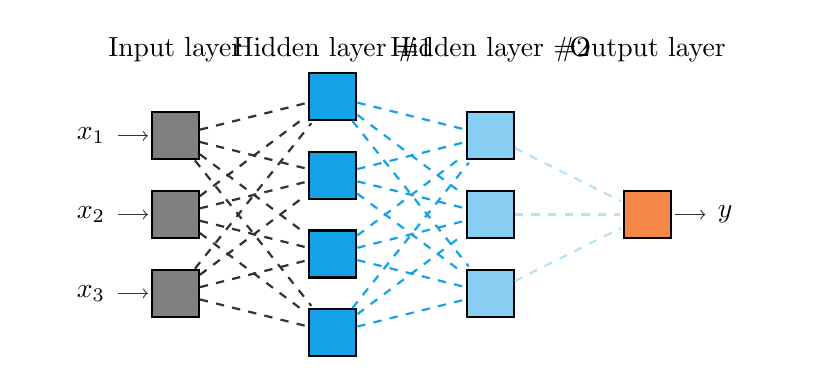
\begin{tikzpicture}[shorten >=1pt,-, draw=black!80, node distance=\layersep]
	\tikzstyle{every pin edge}=[<-,shorten <=1pt]
	\tikzstyle{neuron}=[draw=black, thick, rectangle, minimum size=17pt, inner sep=0pt, thick]
	% \tikzstyle{neuron}=[square, minimum size=17pt, inner sep=0pt, thick]
	\tikzstyle{input neuron}=[neuron, fill=Gray];
	\tikzstyle{output neuron}=[neuron, fill=Peach];
	\tikzstyle{hidden neuron}=[neuron, fill=Cerulean];
	\tikzstyle{hidden neuron2}=[neuron, fill=Cerulean!50];
	\tikzstyle{annot} = [text width=10em, text centered]


	% Draw the input layer nodes
	\foreach \name / \y in {1,...,3}
	% This is the same as writing \foreach \name / \y in {1/1,2/2,3/3,4/4}
	\node[input neuron, pin=left:$x_\y$] (I-\name) at (0,-\y) {};

	% Draw the hidden layer nodes
	\foreach \name / \y in {1,...,4}
	\path[yshift=0.5cm]
	node[hidden neuron] (H-\name) at (\layersep,-\y cm) {};

	% Draw the hidden layer nodes
	\foreach \name / \y in {1,...,3}
	\path[yshift=0.0cm]
	node[hidden neuron2] (H2-\name) at (\layersep+\layersep,-\y cm) {};

	% Draw the output layer node
	\node[output neuron,pin={[pin edge={->}]right:$y$}, right of=H2-2] (O) {};

	% Connect every node in the input layer with every node in the
	% hidden layer.
	\foreach \source in {1,...,3}
	\foreach \dest in {1,...,4}
	\path (I-\source) edge[thick,-,dashed] (H-\dest);
	% \path[path fading=fade IH1, thick, dashed, draw=Gray] (I-\source) -- (H-\dest);


	\foreach \source in {1,...,4}
	\foreach \dest in {1,...,3}
	\path (H-\source) edge[thick,-,dashed,draw=Cerulean] (H2-\dest);
	% \path[path fading=fade H1H2, thick, dashed, draw=Gray] (H-\source) -- (H2-\dest);

	% Connect every node in the hidden layer with the output layer
	\foreach \source in {1,...,3}
	\path (H2-\source) edge[thick,-,dashed,draw=Cerulean!30] (O);
	% \path[path fading=fade H2O, thick, dashed, draw=Gray] (H2-\source) -- (O);

	% Annotate the layers
	\node[annot,above of=H-1, node distance=0.6cm] (hl) {Hidden layer \#1};
	\node[annot,right of=hl] (hl2) {Hidden layer \#2};
	\node[annot,left of=hl] {Input layer};
	\node[annot,right of=hl2] {Output layer};
	\end{tikzpicture}
\end{figure}


	    % \todo{output layers + regularization + works}
	    Particular attention must be paid when fitting deep models as they can be prone to overfit the training set~\cite{angermueller2016deep}.
	    The network topology itself defines the \textit{degrees of freedom} of the model: deeper and wider networks can approximate well very complicated input-output relationship, but also the noise affecting the data.
	    Although, tuning the number of hidden layers and their size is not the recommended strategy to prevent from overfitting, as it may lead to suboptimal solutions.

	    Regularization in MLPs can be controlled by penalizing the weights of the network (see Section~\ref{subsec:regularization_penalties}). The most common regularization strategy consists in adding an $\ell_2$-norm penalty in the objective function, as in Equation~\eqref{eq:losspen}. In the DL community this procedure is known as weight decay~\cite{krogh1992simple}.

	    This strategy is adopted in \cite{Chen2015TransspeciesLO} to train a deep architecture on rat cell responses to given stimuli with the final aim to predict human cell responses in the same conditions.
	    Moreover, weight decay is also adopted in \cite{Yuan2016DeepGeneAA} to train \textit{DeepGene}, \ie an MLP which is designed to classify the tumor type from a set of somatic point mutations.
	    Furthermore, weight decay is used in~\cite{Fakhry2016DeepMF} to train a DL architecture for brain electron microscopy image segmentation.
	    Although less common, the $\ell_1$-norm can also be adopted as regularization penalty, as in~\cite{leung2014deep}.

	    Training MLPs, and deep networks in general, consists in solving a minimization problem via suitable optimization algorithms~\cite{ruder2016overview}. All these methods iteratively update the weights of the network in order to decrease the training error. A popular regularization strategy, known as  \textit{Early stopping}~\cite{prechelt1998early}, consists in interrupting the fitting process as soon as the error on an external validation set increases~\cite{angermueller2016deep}.

	    Another common regularization strategy in DL is \textit{Dropout}~\cite{srivastava2014dropout}. This techniques consists in temporarily deactivating a defined number of randomly chosen units of the network at training phase. This reduces the degrees of freedom of the model and it implicitly allows to achieve an ensemble of several smaller networks whose predictions are combined.
	    The use of dropout alone can improve the generalization properties, as in~\cite{Chen2016GeneEI}, where the authors propose a \textit{D-GEX}, DL regression architecture trained to predict the expression of a number of target genes. Dropout can also be used in combination with weight decay or other forms of regularization, as in~\cite{leung2014deep}, where the authors propose to use a deep network to achieve splicing pattern prediction.

		\begin{table}[htb]
			\centering
			\caption{Overview of the matrix norms used for multiple-output regression.}\label{tab:norms}
			\begin{tabular}{l|l|l}
				\toprule
				Matrix norm  & Notation         & Definition                      \\  \midrule
				Frobenius        & $\norm{A}_F$     & $\sqrt{\text{trace}(A^TA)}$     \\ [0.05cm]
				Nuclear          & $\norm{A}_*$     & $\text{trace}\sqrt{(A^TA)}$     \\ [0.05cm]
				Mixed $\text{L}_{2,1}$        & $\norm{A}_{2,1}$ & $\sum_{j}\norm{\bm{a}_j}_2$ \\ \bottomrule
			\end{tabular}
		\end{table}




  \section{Unsupervised learning} \label{subsec:unsupervised_learning}
    \subsection{Manifold learning}
    \subsection{Clustering}

  \section{Feature selection} \label{subsec:feature_selection}

  \section{Model selection and evaluation} \label{subsec:model_selection}
    \subsection{Model selection strategies}
    % cross validation flavours
    \subsection{Feature selection stability}
    % stability selection
    \subsection{Performance metrics}
    % sup and unsup
    % acc, f1, mcc, ...


\section{Computational requirements and implementations} \label{sec:implementation}
\begin{itemize}
  \item MPI
  \item GPU and accelerators
\end{itemize}
